%!TEX TS-program = pdflatex
%!TEX encoding = UTF-8 Unicode

\documentclass[12pt,a4paper,twoside,english,italian]{book}

\usepackage[utf8]{inputenc}

\usepackage{uniudtesi}

\usepackage[nottoc]{tocbibind}

\usepackage{indentfirst}
\usepackage[ruled,vlined,linesnumbered]{algorithm2e}

\graphicspath{{./figure/}}
\usepackage{amsmath,amsfonts,amssymb,amsthm}
\usepackage{latexsym}
\usepackage{graphicx} % [demo] is just for the example

% \usepackage{natbib}

\newcommand{\N}{\mathbb{N}}
\newcommand{\Z}{\mathbb{Z}}
\newcommand{\Q}{\mathbb{Q}}
\newcommand{\R}{\mathbb{R}}

\newcommand{\C}{\mathbb{C}}

\DeclareMathOperator{\traccia}{tr}
\DeclareMathOperator{\sen}{sen}
\DeclareMathOperator{\arcsen}{arcsen}
\DeclareMathOperator*{\maxlim}{max\,lim}
\DeclareMathOperator*{\minlim}{min\,lim}
\DeclareMathOperator*{\deepinf}{\phantom{\makebox[0pt]{p}}inf}

\newcommand{\varsum}[3]{\sum_{#2}^{#3}\!
   {\vphantom{\sum}}_{#1}\;}
\newcommand{\varprod}[3]{\sum_{#2}^{#3}\!
   {\vphantom{\sum}}_{#1}\;}

%\makeatletter
%\@addtoreset{equation}{section}
%\makeatother
%\renewcommand{\theequation}%
%  {\thesection.\arabic{equation}}

%%%%%%%%%%%%%%%%%%%%%%%%%%%%%%%%%%%%%%%%%%%%%%%%%%%%%%%%%%%

\theoremstyle{plain}
\newtheorem{teorema}{Teorema}[chapter]
\newtheorem{proposizione}[teorema]{Proposizione}
\newtheorem{lemma}[teorema]{Lemma}
\newtheorem{corollario}[teorema]{Corollario}

\theoremstyle{definition}
%\newtheorem{definizione}[teorema]{Definizione}
\newtheorem{definizione}[teorema]{Definition}
\newtheorem{esempio}[teorema]{Example}
\newtheorem{problema}[teorema]{Problem}

\theoremstyle{remark}
\newtheorem{osservazione}[teorema]{Osservazione}

%\usepackage[backend=biber]{biblatex}
%\addbibresource{tesi.bib}

% \usepackage{biblatex}
%\addbibresource{tesi.bib} % with extension

\usepackage{makeidx}
\makeindex

% Ridefiniamo la riga di testa delle pagine:
\usepackage{fancyhdr}
\pagestyle{fancy}
\renewcommand{\chaptermark}[1]{\markboth{#1}{}}
\renewcommand{\sectionmark}[1]{\markright{\thesection\ #1}}
\fancyhf{}
\fancyhead[LE,RO]{\bfseries\thepage}
\fancyhead[LO]{\bfseries\rightmark}
\fancyhead[RE]{\bfseries\leftmark}
\renewcommand{\headrulewidth}{0.5pt}
\renewcommand{\footrulewidth}{0pt}
\setlength{\headheight}{14.5pt}

  \titolo{Similarità di sottografi nelle reti complesse}
  \titoloeng{Subgraph Similarity\\in Complex Networks}
  \laureando{Gaspare Ferraro}
  \annoaccademico{2016-2017}
  \facolta{Scienze Matematiche, Fisiche e Naturali}
  \corsodilaureatriennalein{Informatica}
  \relatore[Prof.]{Roberto Grossi}
  \relatoreDue[Prof.]{Andrea Marino}
  % \dedica{Ai miei genitori\\per non avermi tagliato i viveri}

% Per l'ipertesto:
 \usepackage{hyperref} % gia' caricato da uniudtesi
 \hypersetup{
  bookmarksopen, % default
  bookmarksopenlevel=2, % default;
  pdftitle={Subgraph Similarity in Complex Networks},
  pdfauthor={Gaspare Ferraro},
  pdfsubject={Tesis of Bachelor Degree in Computer Science},
  pdfkeywords={Tesis Bachelor Degree Computer Science Gaspare Ferraro}
  }
  
  \usepackage{listings}
\usepackage{xcolor}
\lstset{language=C++,
                basicstyle=\ttfamily,
                keywordstyle=\color{blue}\ttfamily,
                stringstyle=\color{red}\ttfamily,
                commentstyle=\color{green}\ttfamily,
                morecomment=[l][\color{magenta}]{\#}
}


\begin{document}

\renewcommand{\theequation}{\thechapter.\arabic{equation}}%si torna alle formule numerate come da default
\renewcommand{\thesection}{\thechapter.\arabic{section}}%si torna alle sezioni numerate come da default

\frontmatter

\maketitle

\cleardoublepage

\tableofcontents

% \listoffigures

\mainmatter

% \let\cleardoublepage\clearpage
 
%!TEX TS-program = pdflatex
%!TEX root = tesi.tex
%!TEX encoding = UTF-8 Unicode

\chapter{Introduction}

With the spread of Internet and more importantly of the social networks, efficient data analysis becomes increasingly important.
Graphs are a powerful data structure that model in a natural way information . 

%%%%%%%%%%%%%%%%%%%%%%%%%%%%%%%%%%%%%%%%%%%%%%%%%%%%%%%%%%%%%%%%%%%%%%%%%%%%%%%%%%%%%%%%%%%%%%
%%%%%%%%%%%%%%%%%%%%%%%%%%%%%%%%%%%%%%%%%%%%%%%%%%%%%%%%%%%%%%%%%%%%%%%%%%%%%%%%%%%%%%%%%%%%%%

\section{Basic definitions}

\begin{definizione}\label{def:graph}
    A graph is a pair of sets $G=(V,E)$, where $V$ is the set of vertices (or nodes) and $E \subset V \times V$ is the set of edges.
\end{definizione}

If two vertices $u, v \in V$ are connected by an edge they are called extreme of the edge, in this case we denote the edge with the pair $(u, v) \in E$

If $(u,v) \in E \Leftrightarrow (v,u) \in E$ the graph is called undirected, where not specified we will only deal with undirected graphs.

A sequence of nodes  $v_{1}, v_{2}, \ldots, v_{k}$ is called path if $(v_{i}, v_{i+1}) \in E$ $\forall i = 1, \ldots k-1$; a path is called simple if $v_{i} \neq v_{j}$ $\forall i,j$ $1 \leq i < j \leq k$. A cycle is a path where $(v_{k}, v_{1}) \in E$.

We denote by $N(u) = \{ v : (u,v) \in E \}$ the set of neighbors of the vertex $u$, the cardinality of this set is called degree of $u$ (\textit{deg} $u$ = $|N(u)|)$. 

With $N^{<k}(u)$ we indicate the set of vertex connected to $u$ by a simple path of length less than $k$ (note that $N(u)$ = $N^{<2}(u)$).


\begin{definizione}\label{def:subgraph}
    A graph $G' = (V', E')$ is called subgraph of $G=(V,E)$ if $V' \subset V$ and $E' \subset E$. A subgraph is called induced if $E' = (V' \times V') \cap E$.
\end{definizione}

We use $G' \subset G$ to indicate that the graph $G'$ is a subgraph of $G$ and $G' < G$ to indicate that the graph $G'$ is a induced subgraph of $G$.

Note that an induced subgraph $G' = (V', E')$ can be uniquely identified by the set of its vertex $V'$.\\

\begin{definizione}\label{def:labeledgraph}
	A labeled graph is a triple $(V,E,L)$ where $(V,E)$ is a graph and $L : V \rightarrow \Sigma$
	is a function that assign for every node $v$ a symbol of the alphabet $\Sigma$. We call $L(u) \in \Sigma$ label of the node $u$.
\end{definizione}

Given a path $\pi = v_{1}, v_{2}, \ldots, v_{k}$ we extend the function $L$ and we indicate with $L(\pi) = L(v_{1}) L(v_{2}) \ldots L(v_{k}) \in \Sigma^{k}$ the string obtained by the concatenation of the labels of the nodes in the path.\\

In this thesis we mainly focus to analyze complex network: special graph with a non-trivial topology like random graph. Complex network occur in graphs modelling real system like social networks or computer networks and are characterized by a specific structural features:

\begin{definizione}\label{def:power-law-graph}
	We define as \textit{power-law degree distribution} a networks where the degree of a node $u$ follow, for some $\gamma$ (usualy $2 < \gamma < 3$), the probability:
	\begin{equation}
		P(deg(u) = k) \sim k^{-\gamma}  
	\end{equation}
\end{definizione}

\begin{figure}[h]
	\centering
	\begin{minipage}[t]{.45\textwidth}
		\centering
		
\includegraphics[width=.8\textwidth,height=3.5cm]{figure/cherubino} % TODO
		\caption{Degree distribution of a random network}
	\end{minipage}\hfill
	\begin{minipage}[t]{.45\textwidth}
		\centering
		
\includegraphics[width=.8\textwidth,height=3.5cm]{figure/cherubino} % TODO
		\caption{Degree distribution of a scale-free complex network}
	\end{minipage}
\end{figure}

\begin{figure}[h]
	\centering
	\begin{minipage}[t]{.45\textwidth}
		\centering
		
\includegraphics[width=.8\textwidth,height=3.5cm]{figure/cherubino} % TODO
		\caption{Random network with $|N| = 100$ and $|E| = 1000$}
	\end{minipage}\hfill
	\begin{minipage}[t]{.45\textwidth}
		\centering
		
\includegraphics[width=.8\textwidth,height=3.5cm]{figure/cherubino} % TODO
		\caption{Complex network with $|N| = 100$ and $|E| = 1000$}
	\end{minipage}
\end{figure}
%%%%%%%%%%%%%%%%%%%%%%%%%%%%%%%%%%%%%%%%%%%%%%%%%%%%%%%%%%%%%%%%%%%%%%%%%%%%%%%%%%%%%%%%%%%%%%
%%%%%%%%%%%%%%%%%%%%%%%%%%%%%%%%%%%%%%%%%%%%%%%%%%%%%%%%%%%%%%%%%%%%%%%%%%%%%%%%%%%%%%%%%%%%%%
\section{The problem}

\begin{problema}
Given an undirected labeled graph $G=(V,E,L)$ over an alphabet $\Sigma$, an integer $q$
and two set of nodes $V_{1}, V_{2} \subset V$, we want to estimate the similarity between the two induced subgraphs $V_{1}, V_{2} < G$ based on the labels frequency of simple paths with nodes in $V_{1} \cup N^{<q}(V_{1})$ and $V_{2} \cup N^{<q}(V_{2})$.

\end{problema}

Will discuss about a more formal and rigorous definition of subgraphs similarity in chapter 2.\\

In the definition we use $V_{1} \cup N^{<q}(V_{1})$ and $V_{2} \cup N^{<q}(V_{2})$ instead of simply $V_{1}$ and $V_{2}$ because in a complex graph we also want to keep in mind of the interaction between the subgraph and the external graph.\\

The difficulty we must face is that, in a complex network, the labels can exponentially explode for increasing values of q and $|\Sigma|$ to $|\Sigma|^{q} \gg |V|$ and, even worse, the number of simple paths can exponentially explode to $|V|^{q}$. For the simple reason that in complex networks the average separation is very low (the famous idea of \textit{six degrees of separation}).\\

In this thesis we exploit the problem using randomized techniques and parallelization, which makes the problem suitable even for big network. 

%%%%%%%%%%%%%%%%%%%%%%%%%%%%%%%%%%%%%%%%%%%%%%%%%%%%%%%%%%%%%%%%%%%%%%%%%%%%%%%%%%%%%%%%%%%%%%
%%%%%%%%%%%%%%%%%%%%%%%%%%%%%%%%%%%%%%%%%%%%%%%%%%%%%%%%%%%%%%%%%%%%%%%%%%%%%%%%%%%%%%%%%%%%%%
\section{Pratical applications}

The problem can be applied to a lot of context.
That is why it is very important to choose the right domains for the values of the $V, E, L, \Sigma, q$:
\begin{itemize}
\item $V$ are 
\item $E$ represent the set of interactions, two vertices are connected if exists a relation among them.
\item $L$ and $\Sigma$ are the category that partition $V$, note that if $|\Sigma| = 1$ the labeling is useless.
\item $q$ should be low as $N^{<q}(u)$ could be a large portion of $G$, (e.g. in Facebook for $q \simeq 4$ we have $N^{<q}(u) \simeq G$).
\end{itemize}

Furthermore, we have to choose $G1$ and $G2$ , like ego networks or connected components.\\

% A pratical example: given a social network of people connected by friendship relation, where every people are labeled with their favorite musical genre, estimate the similary, in terms of musical tastes, of two different geographic regions.

 
%!TEX TS-program = pdflatex
%!TEX root = tesi.tex
%!TEX encoding = UTF-8 Unicode

\chapter{Basic tools}

In this chapter we introduce some notion of similarity already existing in literature and then extending them to define similarity among subgraphs in labeled graphs.

In the last sections we present two different techniques we will use afterwards to estimate such similarity.

%%%%%%%%%%%%%%%%%%%%%%%%%%%%%%%%%%%%%%%%%%%%%%%%%%%%%%%%%%%%%%%%%%%%%%%%
%%%%%%%%%%%%%%%%%%%%%%%%%%%%%%%%%%%%%%%%%%%%%%%%%%%%%%%%%%%%%%%%%%%%%%%%
\section{Similarity indices}

\begin{definizione}\label{def:jaccard}
    Given two set $A$ and $B$ we define the \textbf{Jaccard index} as the size of the intersection divided by the size of the union between the two sets:
    
    \begin{equation}
    J(A,B) = \frac{|A \cap B|}{|A \cup B|}
    \end{equation}
    
\end{definizione}

\begin{definizione}\label{def:bray}
    Given two set $A$ and $B$ we define the \textbf{Bray-Curtis index} as:
    
    \begin{equation}
    BC(A,B) = \frac{2 \times |A \cap B|}{|A| + |B|}
    \end{equation}
    
\end{definizione}

\begin{esempio}
	Given $A = \{1, 3, 4, 5, 7, 8\}$ and $B = \{1, 2, 4, 6, 8\}$ we have:
	
	\begin{equation*}
	J(A,B) = \frac{|\{1, 4, 8\}|}{|\{1, 2, 3, 4, 5, 6, 7, 8\}|} = \frac{3}{8} 
	\end{equation*}
	
	\begin{equation*}
	BC(A,B) = \frac{2 \times |\{1, 4, 8\}|}{|\{1, 3, 4, 5, 7, 8\}| + |\{1, 2, 4, 6, 8\}|} = \frac{6}{11} 
	\end{equation*}
\end{esempio}


Note that when $A = B$ we have $J(A,B) = BC(A,B) = 1$ and when $A \cap B = \emptyset$ we have $J(A,B) = BC(A,B) = 0$.

Using sets may be limiting as we consider only once the repeated values, we can easily extended the two previous definition to the multisets.\medskip

\begin{definizione}
	A \textbf{multiset} is a generalization of set that allows multiple instances of elements.
\end{definizione}

To avoid confusion afterwards we use square brackets $[\ ]$ to indicate multiset and curly brackets $\{\ \}$ to indicate set.\medskip

Multiset can also be seen as an array of frequencies of its object (e.g. we indicate with $A = (2, 0, 3)$ the multiset with $2$ elements of first type, $0$ elements of second type and $3$ elements of third type, this notation is equivalent to write $A = [1, 1, 3, 3, 3]$).\medskip

Given two multisets $A = (a_{1}, \ldots, a_{n}) $ and $B = (b_{1}, \ldots, b_{n})$ we define the following operations:

\begin{itemize}
  \item intersection $C = A \cap B  = (c_{1}, \ldots, c_{n})$ where $c_{i} = \min(a_{i}, b_{i})$
  \item union $C = A \cup B  = (c_{1}, \ldots, c_{n})$ where $c_{i} = \max(a_{i}, b_{i})$
  \item multisets union $C = A \uplus B  = (c_{1}, \ldots, c_{n})$ where $c_{i} = a_{i} + b_{i}$
\end{itemize}

% \begin{definizione}\label{def:wjaccard}
%     Given two multisets $A = (a_{1}, \ldots, a_{n}) $ and $B = (b_{1}, \ldots, b_{n})$ we define the \textbf{Frequency Jaccard index} as:
%     
%     \begin{equation}
%     FJ(A,B) = \frac{\sum\limits_{i=1}^n { min(a_{i}, b_{i}) } }{\sum\limits_{i=1}^n { max(a_{i}, b_{i}) }}
%     \end{equation}  
% \end{definizione}


\begin{definizione}\label{def:wbray}
    Given two multisets $A = (a_{1}, \ldots, a_{n}) $ and $B = (b_{1}, \ldots, b_{n})$ we define the \textbf{Bray-Curtis index on multiset} as:
    
    \begin{equation}
    BC(A,B) = \frac{ 2 \times \sum\limits_{i=1}^n { min(a_{i}, b_{i}) } }{\sum\limits_{i=1}^n {a_{i} + b_{i}}}
    \end{equation}
    
\end{definizione}

As a side note, Bray-Curtis is a relevant index for multisets, and is also known as Steinhaus similarity, Pielou's Similarity, Sorensen's quantitative, and Czekanowski's similarity~\cite{legendre1998numerical}.

\begin{esempio}
	Given $A = (0, 2, 3, 1, 0, 3) $ and $B = (2, 0, 1, 3, 1, 2)$ we have:
	
	\begin{equation}
	J(A,B) = \frac{0 + 0 + 1 + 1 + 0 + 2}{2 + 2 + 3 + 3 + 1 + 2} = \frac{4}{13} 
	\end{equation}
	
	\begin{equation}
	BC(A,B) = \frac{2 \times (0 + 0 + 1 + 1 + 0 + 2) }{2 + 2 + 4 + 4 + 1 + 4} = \frac{8}{17}
	\end{equation}
\end{esempio}

Both indices are widely used in practical application, Bray-Curtis index gives a greater weight to the intersection, on the other side the Jaccard Index is a metric and may be preferred to Bray-Curtis index since it is only a semi-metric (as it does not satisfy the triangle inequality). 

\begin{definizione}
	A function $f : A \times A \rightarrow \mathbb{R}^{+} $ is called \textbf{metric} (or simply \textbf{distance}) if satisfy, for all $x, y, z \in A$, the following conditions:
	\begin{itemize}
		\item Non-negativity: $f(x,y) \geq 0$ and $f(x,y) = 0$ iff $x = y$
		\item Symmetry: $f(x, y) = f(y, x)$
		\item Triangle inequality: $f(x, z) \leq f(x, y) + f(y, z)$
	\end{itemize}
\end{definizione}
% \clearpage

%%%%%%%%%%%%%%%%%%%%%%%%%%%%%%%%%%%%%%%%%%%%%%%%%%%%%%%%%%%%%%%%%%%%%%%%
%%%%%%%%%%%%%%%%%%%%%%%%%%%%%%%%%%%%%%%%%%%%%%%%%%%%%%%%%%%%%%%%%%%%%%%%
\section{Documents similarity}

Documents similarity is an hot topic in Information Retrieval, as it can be seen as the problem of duplicate detection~\cite{Broder2000} or, from another point of view, plagiarism detection.\medskip

To define documents similarity we need the notion of \textit{$q$-gram}:

\begin{definizione}
	A \textbf{$q$-gram} is a contiguous subsequence of $q$ items from a sequence.
\end{definizione}

In this case the sequence is a document and the items can be words, characters or even syllables. If the elements used are words, $q$-gram may also be called shingles.

\begin{esempio}
	Given the document \textit{"I live and study in Pisa"} all the possible $3$-grams are: 
	\textit{"I live and"}, \textit{"live and study"}, \textit{"and study in"} and \textit{"study in Pisa"}.
\end{esempio}

Note that in a document with $n$ words the possible $q$-grams are exactly $n-q+1$.\medskip

It is easy to see if we use the set, or multiset, of the all possible $q$-grams of two documents we can use it to calculate their similarity based on the Jaccard or Bray-Curtis index.\medskip

Considering that the number of $q$-grams in a document is linear in its number of words, documents similarity is not an hard problem as we have only to perform union and intersection between set, or multiset.\medskip

\begin{esempio}
	Given the documents 
	\begin{equation*}
	A = \textit{I live, work and study in Pisa}
	\end{equation*}
	\begin{equation*}
	B = \textit{You work and study in Livorno}
	\end{equation*}
	The set of their $2$-grams are:
	\begin{equation*}
	S_{A} = (\textit{I live}, \textit{live work}, \textit{work and}, \textit{and study}, \textit{study in}, \textit{in Pisa})
	\end{equation*}
	\begin{equation*}
	S_{B} = (\textit{You work}, \textit{work and}, \textit{and study}, \textit{study in}, \textit{in Livorno})
	\end{equation*}
	The similarity using both Jaccard and Bray-Curtis are:\medskip
	\begin{equation*}
		J(S_{A},S_{B}) = \frac{|S_{A} \cap S_{B} |}{|S_{A} \cup S_{B} |} = \frac{3}{8}
	\end{equation*}
	\begin{equation*}
		BC(S_{A},S_{B}) = \frac{2 \times |S_{A} \cap S_{B} |}{|S_{A}| +|S_{B}|} = \frac{6}{11}
	\end{equation*}
\end{esempio}

% \clearpage
%%%%%%%%%%%%%%%%%%%%%%%%%%%%%%%%%%%Frequency%%%%%%%%%%%%%%%%%%%%%%%%%%%%%%%%%%%%%
%%%%%%%%%%%%%%%%%%%%%%%%%%%%%%%%%%%%%%%%%%%%%%%%%%%%%%%%%%%%%%%%%%%%%%%%
\section{Graphs similarity}

The definition of similarity between graphs is more complex, as we have to introduce the concept of graph isomorphism.

\begin{definizione}
	A \textbf{graph isomorphism} between two graphs $G=(V_{G}, E_{G})$ and $H=(V_{H}, E_{H})$ is a bijective function from vertices of $G$ to vertices of $H$ that preserve the edge structure, i.e.  
	\begin{equation*}
		f : V_{G} \rightarrow V_{H} \text{ s.t. } (v, u) \in E_{G} \implies (f(v), f(u)) \in E_{H}
	\end{equation*}
\end{definizione}

If such isomorphism exists, the graphs are called isomorphic and we denote it with $G \simeq H$.\medskip

With the notion of graph similarity we can define a similarity between graph~\cite{Bunke:1998:GDM:289720.289729}.

\begin{definizione}
	The similarity between two graphs $G=(V_{G}, E_{G})$ and $H=(V_{H}, E_{H})$ is the size of the largest graph isomorphism between a subgraph $G' \subseteq G$ and a subgraph $H' \subseteq H$ (seen as number of vertex of $G'$).
\end{definizione}

Unfortunately subgraphs isomorphism is a NP-complete problem~\cite{GareyJohnson:1979}, so the only way to solve it is by using heuristic or approximated methods.

% \clearpage 
\begin{esempio}
	\begin{figure}[h]
		\centering
		\begin{minipage}[t]{.45\textwidth}
			\centering
			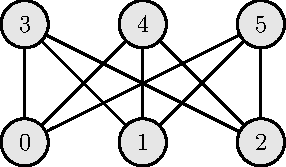
\includegraphics[width=5cm,height=3.33cm]{figure/figure-2-3}
			\caption{Graph $G$}
		\end{minipage}\hfill
		\begin{minipage}[t]{.45\textwidth}
			\centering
			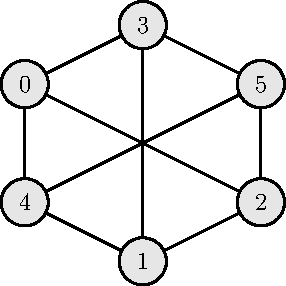
\includegraphics[width=4cm,height=4cm]{figure/figure-2-4}
			\caption{Graph $H$}
		\end{minipage}
	\end{figure}

	The two graphs are isomorphic with the function $f : V_{G} \rightarrow V_{H}$ s.t. $f(0) = 3$, $f(1) = 4$, $f(2) = 2$, $f(3) = 0$, $f(4) = 5$ and $f(5) = 1$. 
	
\end{esempio}


% \clearpage
%%%%%%%%%%%%%%%%%%%%%%%%%%%%%%%%%%%%%%%%%%%%%%%%%%%%%%%%%%%%%%%%%%%%%%%%
%%%%%%%%%%%%%%%%%%%%%%%%%%%%%%%%%%%%%%%%%%%%%%%%%%%%%%%%%%%%%%%%%%%%%%%%
\section{Subgraphs similarity}

After discussing the already existing notions of similarity, we are ready to extend them to define similarity in a labeled complex network.\medskip

Consider a labeled graph $G = (V, E, L)$ over an alphabet $\Sigma$ where $L \rightarrow \Sigma$ is the node labeling, so that each node $u \in V$ has a label $L(u) \in \Sigma$\footnote{Alternatively we can labeling edges in $E$ instead of nodes in $V$ without making too many changes in the following definitions, for sake of simplicity we consider the graph labeled on its nodes.}, we are interest in analyzing $G$ using the sequence of labels in its path.\medskip

For a fixed integer $q > 0$, consider an arbitrary simple path $\pi = u_{1}, \ldots, u_{q}$, we call the orientation $u_{1} \rightarrow \ldots \rightarrow u_{q}$ of $\pi$ a $q$-path leading to $u_{q}$ and $L(\pi) = L(u_{i}) \ldots L(u_{q}) \in \Sigma^{q}$ its $q$-gram, obtained by concatenating the labels of its nodes.\footnote{Note that in an undirected graph we have, for a single simple path, two possible $q$-path, one for each orientation: one leading to $u_{q}$ from $u_{1}$ and one leading to $u_{1}$ from $u_{q}$.}.\medskip

For a set of nodes $A \subseteq V$, we define $L(A)$ as the corresponding multiset of $q$-grams for all $q$-path $\pi$ leading to a node $u \in A$. 
\begin{equation}
L(A) = [x \in \Sigma^{q} : \exists \text{ $q$-path } \pi \text{ leading to } u \in A \text{ with } L(\pi) = x]
\end{equation}

In this way, for each $q$-path $\pi = u_{1}, \ldots, u_{q}$ leading to $u_{q} \in A$, we have that $u_{i} \in A \cup N^{<q}(A)$ $\forall$ $1 \leq i < q$. \medskip

This is a good definition because, as it was mentioned before, we take into account both the internal structure of $A$ and its neighborhood $N^{<q}(A)$. 

Note that we explicitly exclude all the $q$-path both beginning and starting outside $A$, as we not considering them influential to define the similarity.\medskip

Given a single $q$-gram $x$ we are interested in its frequency within the multiset $L(A)$ so we define:
\begin{equation}
	f_{A}[x] = |\{ \pi : \pi \text{ is a $q$-path leading to } u \in A \text{ and } L(\pi) = x \}|
\end{equation}

With the property that $f_{A}[x] = \sum_{u \in A}{f_{\{u\}}[x]}$.

\begin{definizione}
	Given an undirected labeled graph $G = (V,E,L)$ over an alphabet $\Sigma$ and an integer $q > 0$, the Bray-Curtis similarity index between two set of nodes $A, B \subset V$ is:
	\begin{equation}\label{bray-sub}
		BC(A,B) = \frac{ 2 \times \Sigma_{x \in \Sigma^{q}} \min(f_{A}[x], f_{B}[x]) }{ \Sigma_{x \in \Sigma^{q}} f_{A}[x] + f_{B}[x] }
	\end{equation}
\end{definizione}

\begin{definizione}
	Given an undirected labeled graph $G = (V,E,L)$ over an alphabet $\Sigma$ and an integer $q > 0$, the Frequency Jaccard similarity index between two set of nodes $A, B \subset V$ is:
	\begin{equation}\label{jaccard-sub}	
	FJ(A,B) = \frac{ \Sigma_{x \in \Sigma^{q}} \min(f_{A}[x], f_{B}[x]) }{ \Sigma_{x \in \Sigma^{q}} f_{A \cup B}[x] }
	\end{equation}
\end{definizione}

Let $\mathcal{L} = \{ x \in \Sigma^{q} : x \in L(V) \} \subseteq \Sigma^{q}$ be the set of all distinct $q$-grams found in the $q$-paths of G. 

Note that ranging $x$ over $\mathcal{L}$, instead of $\Sigma^{q}$, is sufficient in both the above formulas for any $A$ and $B$.\medskip

In general $BC(A,B) \geq FJ(A,B)$. When $A \cap B = \emptyset$ we have that $f_{A \cup B}[x] = f_{A}[x] + f_{B}[x]$ and $BC(A,B) = 2 \times FJ(A,B)$\medskip

% Note that given two multiset $A = (a_{1}, \ldots, a_{n}) $ and $B = (b_{1}, \ldots, b_{n})$ we define the following operations:

% \begin{itemize}
% 	\item multiset intersection $C = A \cap B  = (c_{1}, \ldots, c_{n})$ where $c_{i} = \min(a_{i}, b_{i})$
% 	\item multiset union $C = A \cup B  = (c_{1}, \ldots, c_{n})$ where $c_{i} = \max(a_{i}, b_{i})$
% 	\item multiset sum $C = A \uplus B  = (c_{1}, \ldots, c_{n})$ where $c_{i} = a_{i} + b_{i}$
% \end{itemize}

%  \clearpage

Now we present a little example to better understand.\medskip

% \begin{figure}[h]
% % 	\centering
% 	\begin{minipage}[t]{.45\textwidth}
% 		\centering
% 		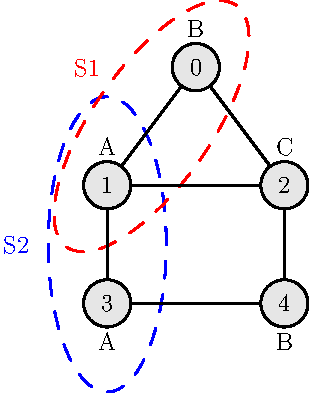
\includegraphics[width=3.9cm,height=5cm]{figure/figure-2-1}
% 	%	\caption{Labeled graph}
% 	\end{minipage}\hfill
% \end{figure}


			\begin{minipage}{0.60\textwidth}\raggedright
			\begin{esempio}
			\end{esempio}
		
			We want to calculate the similarity between the two set $S_{1} = \{0,1\}$ and $S_{2} = \{1, 3\}$ using their $3$-grams of this graph:
		
	\begin{equation*}
L(S_{1}) = [aab, acb, baa, bca, bca, bcb, cab, cba]
\end{equation*}
\begin{equation*}
L(S_{2}) = [baa, baa, bca, bca, caa, cba, cba]
\end{equation*}

% Their union and intersection:
% \begin{equation*}
% L(S_{1}) \cup L(S_{2}) = [aab, acb, baa, baa, bca, bca, bcb, caa, cab, cba, cba]
% \end{equation*}
% \begin{equation*}
% L(S_{1}) \cap L(S_{2}) = [baa, bca, bca, cba]
% \end{equation*}

So we have that:
\begin{equation*}
FJ(S_{1}, S_{2}) = \frac{4}{11} \text{  and  } BC(S_{1}, S_{2}) = \frac{8}{15}
\end{equation*}
			
\end{minipage}
\begin{minipage}{0.30\textwidth}
	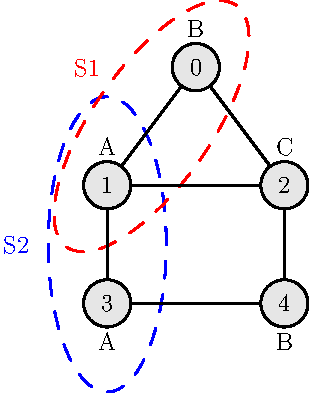
\includegraphics[width=\linewidth]{figure/figure-2-1}
\end{minipage}
	

% \clearpage

%%%%%%%%%%%%%%%%%%%%%%%%%%%%%%%%%%%%%%%%%%%%%%%%%%%%%%%%%%%%%%%%%%%%%%%%
%%%%%%%%%%%%%%%%%%%%%%%%%%%%%%%%%%%%%%%%%%%%%%%%%%%%%%%%%%%%%%%%%%%%%%%%
\section{Sketches}

We have seen that compute the exact similarity between two documents is an easy problem
as we have only to compute the union and the intersection between the two set of shingles.\medskip

More difficult to manage becomes when we have to consider thousands or millions of documents
(e.g. the set of Internet web pages), each one of them has thousands of shingles.\medskip

To solve this problem it is no longer possible to handle all the shingles for all the documents, 
instead we can, for each of them, keep a relatively small, fixed size \textit{sketch}~\cite{Broder2000}.

The computation of the sketches is linear in the size of the documents and can be used to calculate the similarity in linear time in the size of the sketches.\medskip

In the next chapter we will use the sketches applied to the set of $q$-grams of a labeled graph to fast compute the similarity between two subgraphs.\medskip

Usually sketches are used with explicit documents, we will use it to avoid to generate all the $q$-grams.\medskip

Now we present two different existing technique to compute the sketches of a document, 
for simplicity we assume that our document is composed by all numbers between $1$ and $n$, 
in practice we will use a ranking function to define a sorting to the elements in documents.

%%%%%%%%%%%%%%%%%%%%%%%%%%%%%%%%%%%%%%%%%%%%%%%%%%%%%%%%%%%%%%%%%%%%%%%%
%%%%%%%%%%%%%%%%%%%%%%%%%%%%%%%%%%%%%%%%%%%%%%%%%%%%%%%%%%%%%%%%%%%%%%%%
\subsection*{Min-wise permutation}

The first approach to compute a sketch of a document is the min-wise permutation~\cite{Broder:1998:MIP:276698.276781}.\medskip

Given a document $A = \{1, \ldots, n\}$, to calculate its sketch $S_{A}$ of size $k$ 
we choose $k$ random independent permutation $\pi_{i} : \{1, \ldots, n\} \rightarrow \{1, \ldots, n\}$ and define the sketch as:

\begin{equation*}
	S_{A} = \{ \min(\pi_{1}(A)), \ldots, \min(\pi_{k}(A)) \}
\end{equation*}

Note that using the min-wise permutation we can take multiple times the same number, as the permutation are independent.

\clearpage
%%%%%%%%%%%%%%%%%%%%%%%%%%%%%%%%%%%%%%%%%%%%%%%%%%%%%%%%%%%%%%%%%%%%%%%%
%%%%%%%%%%%%%%%%%%%%%%%%%%%%%%%%%%%%%%%%%%%%%%%%%%%%%%%%%%%%%%%%%%%%%%%%
\subsection*{Bottom-k sketches}

Another approach that works best in terms of performance is the bottom-k sketches~\cite{Cohen:2007:SDU:1281100.1281133}.\medskip

Instead of using $k$ random permutation $\pi_{1}, \ldots, \pi_{k}$ and take the minimum for each of them,
like we did before in the min-wise permutation, we choose only one random permutation $\pi$ and take the bottom $k$ elements with lower value in permutation.

\begin{equation*}
S_{A} = \{ \min_{1}(\pi(A)), \ldots, \min_{k}(\pi(A)) \}\footnote{With $\min_{x}$ we indicate the x-minimum element}
\end{equation*}

Note that, unlike the min-wise permutation, in the bottom-k sketches we don't have repeated numbers as we take the numbers from a single permutation.

\begin{esempio}
	Consider the document $A=\{1, \ldots, 10\}$ and the following $4$ permutation ($k = 4$):
	
	\begin{equation*}
		\pi_{1} = \{3, 5, 8, 2, 4, 9, 1, 10, 7, 6\}
	\end{equation*}
	\begin{equation*}
		\pi_{2} = \{7, 10, 2, 1, 8, 5, 9, 6, 4, 3\}
	\end{equation*}
	\begin{equation*}
		\pi_{3} = \{3, 4, 6, 2, 8, 5, 1, 10, 7, 9\}
	\end{equation*}
	\begin{equation*}
		\pi_{4} = \{9, 1, 3, 5, 4, 10, 7, 8, 2, 6\}
	\end{equation*}
	
	With the min-wise permutation approach we have that:
	\begin{equation*}
		S_{A} = \{ \min(\pi_{1}(A)), \min(\pi_{2}(A)), \min(\pi_{3}(A)), \min(\pi_{4}(A)) \} = \{3, 7, 3, 9\}
	\end{equation*}
	
	Instead with the bottom-k sketches using $\pi_{4}$ as permutation:
	\begin{equation*}
	S_{A} = \{ \min_{1}(\pi_{4}(A)), \min_{2}(\pi_{4}(A)), \min_{3}(\pi_{4}(A)), \min_{4}(\pi_{4}(A)) \} = \{9, 1, 3, 5\}
	\end{equation*}
	
\end{esempio}


%%%%%%%%%%%%%%%%%%%%%%%%%%%%%%%%%%%%%%%%%%%%%%%%%%%%%%%%%%%%%%%%%%%%%%%%
%%%%%%%%%%%%%%%%%%%%%%%%%%%%%%%%%%%%%%%%%%%%%%%%%%%%%%%%%%%%%%%%%%%%%%%%
\section{Color Coding}

The color coding is a method proposed in 1994 by Alon et al.~\cite{Alon:1995:COL:210332.210337} that efficiently finds simple path, cycles or many other small subgraphs using probabilistic algorithm. We will focus only to finds $q$-simple paths.\medskip

The idea behind this method, which gives it the name, is to randomly coloring each node of $V$ with one of the $q$ possible color.

We restrict our attention to $q = O(\log |V|)$ and denote with $\chi : V \rightarrow [q]$\footnote{Where $[q] \equiv [1, \ldots, q]$ is the set of all possible colors} the coloring function, where each node $u \in V$ have a color $\chi(u) \in [q]$.\medskip

After assigning a color to each node, we will focus to find only the colorful $q$-paths. We say that a $q$-path $u_{1}, \ldots, u_{q}$ is colorful iff $\chi(u_{i}) \neq \chi(u_{j})$ for $1 \leq i < j \leq q$ (i.e. all the $q$ colors appear in the $q$-path).\medskip

The main advantage of this method is that reduce the number of $q$-paths by roughly a factor of $q! / q^{q} \geq 1/e^{q}$, as a colorful $q$-path can use $q!$ colorings of its nodes out of $q^{q}$ possible ones. So the number of $q$-paths exponentially decrease as the value of $q$ increases, when $q = 3$ we look only for the $\sim22\%$ colorful $q$-paths and only for $\sim4\%$ when $q = 5$.\medskip

As we will show in the next chapter, all the colorful $q$-paths can be easily found using a dynamic programming approach.\medskip

An interesting fact is that the method of color coding can be derandomized using a $k$-perfect hash family~\cite{Alon:1995:COL:210332.210337}, that enumerating all the possible $k$-colorings of $V$.
This makes the method exponential in the value of $q$, as if we set $q = |V|$ the problem became to find an Hamiltonian path, which is NP-complete~\cite{GareyJohnson:1979}.\medskip

To improve precision we can repeat the random coloring of nodes for $e^{q}\ t$ times, 
so that success probability becomes $\geq 1-e^{-t}$. 
Another way is to random coloring nodes using a greater number of colors $q'$ and then, instead of looking for the colorful $q'$-paths,
we search the color-diversified $q$-paths (i.e. $q$-paths without color repetition in $[q']$)~\cite{deshpande2007randomized}.\medskip

In practice, choosing a simple random coloring is working pretty well on complex networks, 
so for don't add overhead to our algorithms we won't utilize the previous optimizations .\medskip


	\begin{minipage}{0.55\textwidth}\raggedright
		\begin{esempio}
		\end{esempio}
		
		In this $3$-colored graph out of $6$ simple $3$-path starting from $0$\medskip
		
		($\textsc{0-1-2}$ $\textsc{0-1-3}$ $\textsc{0-2-1}$ $\textsc{0-2-4}$ $\textsc{0-2-6}$ $\textsc{0-5-6}$)\medskip
		
		only $3$ are colorful ($\textsc{0-1-2}$ $\textsc{0-2-1}$ $\textsc{0-2-4}$).
	\end{minipage}
	\begin{minipage}{0.35\textwidth}
		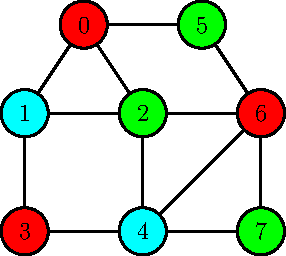
\includegraphics[width=\linewidth]{figure/figure-2-6}
	\end{minipage}

\noindent

\clearpage

 
\chapter{Computation of subgraph similarity}

In this chapter, we present four different theoretical algorithms to compute subgraphs similarity as previously defined: an exhaustive enumeration, two similar randomized approaches using the tools described in the previous chapter, and a naive randomized approach as a baseline for comparison.\medskip
	
In the following algorithms, we will make use of parallel instructions, postponing the specific programming choices and the comparison among the different approaches to the next chapter.
	
\section{Indices computation}

Now we illustrate the algorithms to calculate the Frequency Jaccard and Bray-Curtis indices, as they are independent from the next algorithms we will present.\bigskip

As previously seen, instead of iterating over all the strings in $\Sigma^{q}$ we can restrict to $\mathcal{L} \subseteq \Sigma^{q}$, which is the set of all possible $q$-grams found in the $q$-paths of $G$.\medskip 

An additional improvement can be made as follows. If we want to compute the similarity between two set $A, B \subset V$, it is enough to ranging, instead over $\mathcal{L}$, over $\mathcal{W} = \{ x \in \Sigma^{q} : x \in L(A) \text{ or } x \in L(B) \} \subseteq \Sigma^{q}$, as we can easily see that for any $x \in ( \Sigma^{q} \setminus \mathcal{W} )$ both $f_A[x]$ and $f_B[x]$ are equal to zero.\bigskip

Also, we can observe that in the Frequency Jaccard index we do not have to explicitly calculate $f_{A \cup B}[x]$ and its sketch, as the exact value of $R = \Sigma_{x \in \mathcal{W}} f_{A \cup B}[x]$ can be easily calculated from $f_{A}[x] \text{ and } f_{B}[x]$.\bigskip

So we define the following procedures based on \eqref{bray-sub} and \eqref{jaccard-sub}.\medskip

\begin{algorithm}[h]
	\small
	\DontPrintSemicolon
	\SetKwInOut{Input}{Input}
	\SetKwInOut{Output}{Output}
	\Input{$\mathcal{W} = $ dictionary of $q$-grams\\$f_{A}[x] = $ frequency of each $x \in \mathcal{W}$ in $A$\\$f_{B}[x] = $ frequency of each $x \in \mathcal{W}$ in $B$}
	\Output{$BC(A,B) = $ the similarity between $A$ and $B$ according to Bray-Curtis index}
	\BlankLine
	$num \gets 0$\;
	$den \gets 0$\;
	\ForEach{$x \in \mathcal{W}$}{
		$num \gets num + 2 \times \min( f_{A}[x], f_{B}[x] )$\;
		$den \gets den + f_{A}[x] + f_{B}[x]$\;
	}
	$BC \gets \frac{num}{den}$\;
	\Return{$BC$}
	\caption{\textsc{Bray-Curtis}}
	\label{alg:bray-curtis}
\end{algorithm}

\begin{algorithm}[h]
	\small
	\DontPrintSemicolon
	\SetKwInOut{Input}{Input}
	\SetKwInOut{Output}{Output}
	\Input{$\mathcal{W} = $ dictionary of $q$-grams\\$f_{A}[x] = $ frequency of each $x \in \mathcal{W}$ in $A$\\ $f_{B}[x] = $ frequency of each $x \in \mathcal{W}$ in $B$\\ $R =$ summation of all frequency}
	\Output{$FJ(A,B) = $ the similarity between $A$ and $B$ according to Frequency Jaccard index}
	\BlankLine
	$num \gets 0$\;
	\ForEach{$x \in \mathcal{W}$}{
		$num \gets num + \min( f_{A}[x], f_{B}[x] )$\;
	}
	$FJ \gets \frac{num}{R}$\;
	\Return{$FJ$}
	\caption{\textsc{Frequency-Jaccard}}
	\label{alg:jaccard}
\end{algorithm}

Algorithm \ref{alg:bray-curtis} and \ref{alg:jaccard} compute the values of $BC(A,B)$ and $FJ(A,B)$, as previously defined, by ranging over the given dictionary of $q$-grams $\mathcal{W}$.

\begin{lemma}
	The execution of \textsc{Bray-Curtis} or \textsc{Frequency-Jaccard} requires $O(|W|)$ time and $O(1)$ space. 	
\end{lemma}

In the next algorithms, we will only focus to compute the values of $\mathcal{W}$, $f_{A}$, $f_{B}$ and $R$.

\clearpage 

\section{Naive approach}

The naive approach consists in enumerating all the possible $q$-grams of simple $q$-paths leading to $u \in A \cup B$. This can be done by starting an exhaustive search for each $u \in A \cup B$.
	
\begin{algorithm}[h]
	\small
	\DontPrintSemicolon
	\SetKwInOut{Input}{Input}
	\SetKwInOut{Output}{Output}
	\Input{$q = $ length of the paths\\$A, B = $ set of nodes to compare}
	\Output{$\mathcal{W} = $ dictionary of $q$-grams\\$f_{A}[x] = $ frequency of each $x \in \mathcal{W}$ in $A$\\ $f_{B}[x] = $ frequency of each $x \in \mathcal{W}$ in $B$\\ $R =$ summation of all frequency}
	\BlankLine
	$R \gets 0$\;
	$\mathcal{W} \gets \emptyset$\;
	$f_{A \cup B} \gets \emptyset$ \quad \;    
	$f_{A} \gets \emptyset$\; 
	$f_{B} \gets \emptyset$\; 
	\BlankLine
	\textbf{parallel} \ForEach{$u \in A \cup B$}{
		$\langle \mathcal{W}_{u}, f_{u} \rangle \gets \textsc{ExhaustiveSearch}(\langle u \rangle, q)$\;
		$\mathcal{W} \gets \mathcal{W} \cup \mathcal{W}_{u}$\;
		$f_{A \cup B} \gets f_{A \cup B} \cup f_{u}$\;
	}
	\BlankLine    
	\ForEach{$\langle u, x \rangle \in f_{A \cup B}$}{ 
		$R \gets R + f_{A \cup B}[\langle u, x \rangle]$\;
		\If{$u \in A$}{
			$f_{A}[x] \gets f_{A}[x] + f_{A \cup B}[\langle u, x \rangle]$\;
		}
		\If{$u \in B$}{
			$f_{B}[x] \gets f_{B}[x] + f_{A \cup B}[\langle u, x \rangle]$\;
		}
	}
	\BlankLine
	\Return{$\langle \mathcal{W}$, $f_{A}$, $f_{B}$, $R \rangle$}
	\caption{\textsc{brute-force}}
	\label{alg:brute-force}
\end{algorithm}

Here we define $\mathcal{W}_{u}$ and $f_{u}$ as, respectively, the dictionary and the frequency of $q$-grams of the $q$-paths leading to the node $u \in A \cup B$.
	 
Thus we compute $\mathcal{W}$ with the property $\mathcal{W} = \Sigma_{u \in A \cup B}{\ \mathcal{W}_{u} }$ and, in the same way, $f_{A \cup B}$ with the property $f_{A \cup B} = \Sigma_{u \in A \cup B}{\ f_{u} }$.
	
The value of $R$ is computed as described at the beginning of the chapter, namely, $R = \Sigma_{x \in \mathcal{W} }{\ f_{A \cup B}[x] }$.

At last, we can compute the value of $f_{A}$ and $f_{B}$ from $f_{A \cup B}$ by looking at the leading nodes and separate the frequencies, depending if it belongs to $A$, $B$ or both.

Note that, as we have to separate the frequencies between $f_{A}$ and $f_{B}$, the type of $f_{A \cup B}$ is not a mapping $ \Sigma^{q} \rightarrow \mathbb{N}$ but instead is a mapping $V \times \Sigma^{q} \rightarrow \mathbb{N}$, where the element in $V$ is the leading node of the $q$-path associated with the $q$-gram.\medskip
	
The values of $FJ(A,B)$ and $BC(A,B)$ computed using this method are exact, and we will use it only to evaluate the precision of the other approaches, as it requires to examine all the possible $O(|\Sigma|^{q})$ $q$-gram with a complexity of $O(|V|^{q})$.\medskip
	
For completeness, we also illustrate the $\textsc{ExhaustiveSearch}$ algorithm that keeps track of the current $q$-path and its relative $q$-gram.
	
\begin{algorithm}[h]
	\small
	\DontPrintSemicolon
	\SetKwInOut{Input}{Input}
	\SetKwInOut{Output}{Output}
	\Input{$\pi = \langle u_{1}, \ldots, u_{|\pi|} \rangle $ current traversing path of length $\leq q$ \\$q = $ length of the paths }
	\Output{$\mathcal{W} =$ dictionary of $q$-grams of $q$-path having $\pi$ as suffix\\$f_{u}[\langle u_{q}, x \rangle] = $ frequency of each $x \in \mathcal{W}$ leading to $u_{q}$}
	\BlankLine
	$\mathcal{W} \gets \emptyset$\;
	$f_{u} \gets \emptyset$ \quad \;    
	\BlankLine
	\If{$|\pi| = q$}{
		$\mathcal{W} \gets \{ L(\pi) \}$\;
		$f_{u}[\langle u_{q}, L(\pi) \rangle] \gets 1$\;
	}
	\Else{
		\ForEach{$v \in N(u_{1}) \setminus \pi$}{
			$\langle \mathcal{W}_{v}, f_{v} \rangle \gets \textsc{ExhaustiveSearch}(\langle v \rangle \cdot \pi, q)$\;
			$\mathcal{W} \gets \mathcal{W} \cup \mathcal{W}_{v}$\;
			$f_{u} \gets f_{u} \cup f_{v}$\;
		}	
	}
	\BlankLine
	\Return{$\langle \mathcal{W}$, $f_{u} \rangle$}
	\caption{$\textsc{ExhaustiveSearch}$}
	\label{alg:exhaustive-search}
\end{algorithm}

Here the symbol $\cdot$ is the concatenation of the paths. Note that we put the node $v$ before the path $\pi$ as we are interested to find all the $q$-paths leading to the node $u$.\medskip
	
In Algorithm \ref{alg:exhaustive-search}, when $\pi$ is a $q$-path, we have the base case of the recursion that simply returns $\mathcal{W} = \{ L(\pi) \}$, which is the dictionary composed only by the label of $\pi$, and the frequency $f_{u}[\langle u_{q}, L(\pi) \rangle] = 1$ as we have only one path.
	
When the path $\pi$ is shorted than $q$, we recursively visit all its neighbors, with the new path obtained by prepending the node $v$ to the current path $\pi$.\medskip
	
\clearpage
	
Finally, using $N(u_{1}) \setminus \pi$ we avoid to traverse again the nodes already in the path $\pi$. In this way we restrict the searching only to the simple $q$-paths.
	
\begin{lemma}
	For any two sets of nodes $A, B \subseteq V$, the running time of \textsc{brute-force} requires $O(|V|^{q})$ time and $O(\mathcal{L}) = O(|\Sigma|^{q})$ space.
\end{lemma}

Now we present a little example to better understand our ideas.
	
\begin{esempio}
	We want to compute the similarity between the two nodes $4$ and $3$ in the following graph.	
\end{esempio}

\begin{wrapfigure}{R}{0\textwidth}
	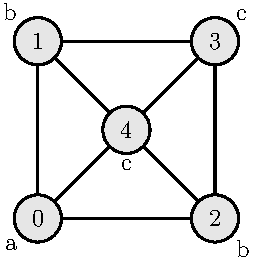
\includegraphics[width=0.35\textwidth]{figure/figure-3-2}
\end{wrapfigure}
	
$\textsc{ExhaustiveSearch}(4, 3)$ returns \medskip

$\mathcal{W}_{4} = \{ abc, bac, bcc, cbc \}$ \medskip
		
$f_{4}[\langle 4, abc \rangle] = 2$ ($\textsc{0-1-4}$ $\textsc{0-2-4}$)\medskip
		
$f_{4}[\langle 4, bac \rangle] = 2$ ($\textsc{1-0-4}$ $\textsc{2-0-4}$)\medskip
		
$f_{4}[\langle 4, bcc \rangle] = 2$ ($\textsc{1-3-4}$ $\textsc{2-3-4}$)\medskip
		
$f_{4}[\langle 4, cbc \rangle] = 2$ ($\textsc{3-1-4}$ $\textsc{3-2-4}$)\bigskip
		
$\textsc{ExhaustiveSearch}(3, 3)$ returns\medskip
		
$\mathcal{W}_{3} = \{ abc, acc, bcc, cbc \}$\medskip
		
$f_{3}[\langle 3, abc \rangle] = 2$ ($\textsc{0-1-3}$, $\textsc{0-2-3}$)\medskip
		
$f_{3}[\langle 3, acc \rangle] = 1$ ($\textsc{0-4-3}$)\medskip
		
$f_{3}[\langle 3, bcc \rangle] = 2$ ($\textsc{1-4-3}$, $\textsc{2-4-3}$)\medskip
		
$f_{3}[\langle 3, cbc \rangle] = 2$ ($\textsc{4-1-3}$, $\textsc{4-2-3}$)\bigskip
		
So the dictionary $\mathcal{W}$ is \medskip
		
$\mathcal{W} = \mathcal{W}_3 \cup \mathcal{W}_4 = \{ abc, acc, bac, bcc, cbc \}$\bigskip
		
The similarity according to the two indices is \medskip

$BC(\{3\}, \{4\}) = \frac{2 \times (2 + 0 + 0 + 2 + 2) }{4 + 1 + 2 + 4 + 4} = \frac{12}{15}$ \medskip
		
$FJ(\{3\}, \{4\}) = \frac{2 + 0 + 0 + 2 + 2}{4 + 1 + 2 + 4 + 4} = \frac{6}{15}$ \medskip
		
\clearpage

\section{Efficient computation}

The main hurdle of our problem is to compute the frequency mapping $f_{X}[\ ]$ for some sets $X \in V$, as it can grow up to a size of $|\Sigma|^{q}$, and its definition requires to explore potentially $|V|^{q}$ $q$-paths.\medskip

We present a random unbiased estimator based on color coding and sketching with the property that it can be computed efficiently even on large networks, and its expected value is the actual similarity index~\cite{SubSim}.\medskip

First, using the color coding we reduce the number of potentially explored $q$-paths from $|V|^{q}$ to $2^{O(q)}|V|$, thus making it feasible for large values of $|V|$, assuming $q = O(\log |V|)$.

Second, instead of calculating the correct value of $f_{X}$, we compute its sketch with a size small compared to $|\Sigma|^{q}$, which is a significant benefit when $|\Sigma|$ or $q$ are large.

\subsection*{$preprocess(G,q)$: Color coding of the $q$-paths}

Now we illustrate how to preprocess the input graph $G=(V,E)$ given an integer $q > 0$, in particular, where $q = O(\log |V|)$.

Note that the preprocessing task is performed independently from the choice of the labeling function $L$ and the subsets $A,B$ to compare. It depends only on the graph $G$ and the value of $q$, so we can execute the preprocessing once and then reuse the same color coding table for different values of $A,B$ or even $L$.\medskip

\begin{algorithm}[h]
		
	\small
	\DontPrintSemicolon
	\SetKwInOut{Input}{Input}
	\SetKwInOut{Output}{Output}
	\Input{$G = (V,E)$ undirected graph with $q$ random colors.}
	\Output{$M = $ dynamic programming table for color coding.}
	\BlankLine
	\textbf{parallel} \lForEach{$u \in V$}{$M_{1,u} = \langle \chi(u), 1 \rangle$}
	\BlankLine
	\For{$i \in \{ 2, 3, \ldots, q\}$}{
		\textbf{parallel} \ForEach{$u \in V$}{
			\ForEach{$v \in N(u)$}{
				\ForEach{$\langle C, f \rangle \in M_{i-1,v}$ such that $\chi(u) \not \in C$}{
					$f' \gets M_{i,u}\left(C \cup \{\chi(u)\}\right)$\;
					$M_{i,u} \gets \langle C \cup \{\chi(u)\}, f' + f \rangle$\;
				}
			}
		}   
	}
	\Return{$M$}	
	\caption{$\textsc{preprocess}$: $\textsc{color-coding}$}
	\label{alg:color-coding}
\end{algorithm}

The next goal is to list all the colorful $q$-paths in $G$ using a dynamic programming approach.\medskip

First of all we assign a random coloring $\chi : V \rightarrow [q]$, so that each node $u \in V$ has a color $\chi(u)$ independently and uniformly chosen from $[q]$. Algorithm \ref{alg:color-coding} build and return a table $M$ of size $q \times |V|$ where $M_{i,j}$ stores the collection of pairs $\langle C, f \rangle$ where  $C \subseteq [q]$ is a color set such that $|C| = i$ and there are $f$ colorful $i$-paths leading to the node $j$.\medskip

Our assumption that $q = O(\log |V|)$ allows us to implement, using bit manipulations, operations on color sets in $O(1)$ time as they fit in a machine words.\medskip

Note that each entry $M_{i, j}$ contains at most $\binom{q}{i}$ sets, each with $i$ colors. Hence the computation of the row $i$ can be done in parallel as it depends only from the row $i-1$ and require $O(|E|\ \binom{q}{i-1})$ time (as we scan all the adjacency list). The entire computation requires thus $O(|E|\ \Sigma_{i=1}^{q}{\binom{q}{i-1}}) = O(|E|\ 2^{q})$ time.\bigskip

For what concern space, the table $M$, as we already said, has a total of $q \times |V|$ entries, each of which contains at most $\binom{q}{i}$ pairs $\langle C, f \rangle$.

Each pair can be stored in $O(1)$ as they are simply $2$ integer, we have a total size of $O(\Sigma_{i=1}^{q}{\Sigma_{j=1}^{|V|}{ \binom{q}{i}}}) = O(|V|\ \Sigma_{i=1}^{q}{\binom{q}{i}}) = O(|V|\ 2^{q})$.\bigskip

\begin{lemma}
	Given an undirected graph $G=(V, E)$ random colored in $[q]$, where $q = O(\log |V|)$, Algorithm \ref{alg:color-coding} (preprocess($G$,$q$)) returns the dynamic programming table $M$ of color coding in $O(|E|\ 2^{q})$ time and $O(|V|\ 2^{q})$ space. 
\end{lemma}

\bigskip

It is not difficult to modify the Algorithm \ref{alg:color-coding} to list also the colorful $q$-grams, printing $L(\pi)$ for each colorful $q$-path $\pi$. This makes the algorithms inefficient, indeed we still have to face with the problem that $\mathcal{L} \sim \Sigma^{q}$.\bigskip

So we will pass to the next step.

\subsection*{$query(A,B)$: Sampling and sketching colorful paths}

Now using the color coding table $M$, and given two set of nodes $A, B$, we want to approximate the values of $BC(A,B)$ and $FJ(A,B)$.\bigskip

As already said, we cannot explore all the colorful $q$-grams, so our idea is to construct a sample of $\mathcal{L}$, without explicitly calculate it, by sampling $r$ $q$-paths from $M$, where $r < |\mathcal{L}|$ is a user-selectable parameter.

We will use as a sample $r$ $q$-paths  without repetition. This can be also seen as a bottom-r sketch of all the $q$-paths.\bigskip 

\clearpage

Our algorithm for $\textsc{query}(A,B)$ consist of three phases as follows:

\begin{itemize}
	\item Compute a suitable sketch $W \subset \mathcal{L}$ such that $\tau = |W|$ is at most $r$, by sampling $r$ colorful $q$-paths using $M$ and setting $W$ as the sets of the $q$-grams of these paths.
	\item Compute $f_{A}[x]$, $f_{B}[x]$ for each $x \in W$.
	\item Approximate $BC(A,B)$ as $BC_{W}(A,B)$ and $FJ(A,B)$ as $FJ_{W}(A,B)$.
\end{itemize}

Where $BC_{W}(A,B)$ and $FJ_{W}(A,B)$ are defined as:

\begin{equation}\label{bc-w}
	BC_{W}(A,B) = \frac{ 2 \times \Sigma_{x \in W} \min(f_{A}[x], f_{B}[x]) }{ \Sigma_{x \in W} f_{A}[x] + f_{B}[x] }
\end{equation}

\begin{equation}\label{fj-w}
	FJ_{W}(A,B) = \frac{ \Sigma_{x \in W} \min(f_{A}[x], f_{B}[x]) }{ \Sigma_{x \in W} f_{A \cup B}[x] }
\end{equation}

\subsection*{Phase 1: Colorful sampler}

Sampling uniformly using a dynamic programming approach is a topic already covered in the literature, e.g. Martin Dyer in ~\cite{Dyer:2003:ACD:780542.780643} or Eric Vigoda in ~\cite{Vigoda2010LectureNO}. In particular, we are interested in sampling $\tau$ $q$-grams from colorful $q$-paths, leading to nodes belonging to $X$, using the color coding table $M$.\bigskip

As we are dealing with weighted sets (where the weights are frequencies), the sample must depend on the frequencies of the $q$-grams ending in $x \in X$, as in the case of consistent weighted sampling, where more frequent $q$-grams need to be sampled more often.
 
As we do not know a priori the frequency of $q$-grams before sampling, we sample $q$-paths uniformly at random so that the probability of getting a $q$-gram is proportional to the number of paths having that $q$-gram, i.e. its frequency. The uniform sampling of paths can be done by looking at the frequencies of colorful $q$-paths in $M$. We know that the number of colorful $q$-paths ending in $v$ is $M_{q,v}([q])$, hence we extract the starting node $x \in X$ of our weighted random $q$-paths with a probability:\bigskip

\begin{equation}
	p_{X}(v) = \frac{ M_{q,v}([q]) }{ \Sigma_{x \in X}{M_{q, x}([q])} }
\end{equation}

\bigskip

Then we generate a random $q$-path by scanning the color coding table $M$ backward from $q-1$ to $1$, choosing nodes with a probability similar to $p_{X}(v)$ (except that during step $i$ we look at row $i$ and in the complementary of the color set of the current $i$-path).\bigskip

\clearpage

We define out sampling algorithm as shown in Algorithm~\ref{alg:colorful-sampler}.

\begin{algorithm}[h]
	\small
	\DontPrintSemicolon
	\SetKwInOut{Input}{Input}
	\SetKwInOut{Output}{Output}
	\Input{$X =$ multiset of nodes from graph $G$\\$M =$ color coding table for $G$\\$r$ number of colorful paths to sample.}
	\Output{$W = $ random sample composed by $q$-grams of $q$-paths leading to $x \in X$}
	\BlankLine
	$R \gets \{\}$\;
	\BlankLine
	\textbf{parallel} \For{$j\in [r]$}{
		$u\gets$ randomly chosen $v \in X$ with probability~$p_v = \frac{M_{q,v}([q])}{\sum_{z\in X} M_{q,z}([q])}$\label{line:sample}\;
		$\pi\gets \textsc{random-path-to}(u)$\;
		\lIf{$\pi\not\in R$}{$R \gets R \cup \{ \pi \}$}
		\lElse{$j\gets j-1$ \quad //repeat the step}
	}
	\BlankLine
	\Return{$W = \{ L(\pi) : \pi \in R \}$}
	\BlankLine
	\caption{$\textsc{colorful-sampler}$}
	\label{alg:colorful-sampler}
\end{algorithm}

The procedure $\textsc{random-path-to}$ is defined in Algorithm~\ref{alg:random-path-to}.

\begin{algorithm}[h]
	\small
	\DontPrintSemicolon
	\SetKwInOut{Input}{Input}
	\SetKwInOut{Output}{Output}
	\Input{$M =$ color coding table for $G$\\$u = $ leading node of the path }
	\Output{$\pi = $ random colorful path }	
	$P\gets \langle u \rangle$\;
	$D\gets [q] \setminus \{\chi(u)\}$\;
	\For{$i \in \{q-1,\ldots, 1\}$}{
		$u\gets$ randomly chosen $v \in N(u)$ with probability~$p_{v} = \frac{M_{i,v}(D) }{ \sum_{z\in N(u)} M_{i,z}(D)}$\;
		$P\gets u \cdot P$\;
		$D\gets D\setminus \{\chi(u)\}$\;
	}
	\Return{P}   
	\caption{$\textsc{random-path-to}$}
	\label{alg:random-path-to}
\end{algorithm}

Note that the method $\textsc{random-path-to}$ always finds a colorful $q$-path, as at each step we choose nodes only among the ones that will lead to a colorful $q$-path (i.e. the probability $p_{v}$ is $0$ for nodes that don't lead to a colorful $q$-path). This property is guaranteed by the way the color coding table $M$ is generated by Algorithm \ref{alg:color-coding}.

\begin{lemma}
	For any multiset of nodes $X$, 
	Algorithm \ref{alg:colorful-sampler} returns a random sample $W \subset |\Sigma^{q}|$ with a complexity of $O(rq)$ both in time and space, 
	where $q = O(\log |V|)$ and $r < |\mathcal{L}| \leq |\Sigma|^{q}$.
\end{lemma}

\clearpage
\subsection*{Phase 2: Frequency count}

Now that we have a sample $W$, of suitable size, composed by $q$-grams, we are interested, for a multiset of nodes $X$, in calculating $f_{X}[x]$ for each $x \in W$. Algorithm~\ref{alg:f-count}, for steps $i = 1, 2, \ldots, q$, proceeds by expanding in $BFS$ order only the $i$-paths ending in a node $u \in X$ and having $i$-grams that are suffixes of $W$ (this operation can be made more space efficient by using tries or by performing a binary search in a set of strings).\medskip

We maintain a multiset $T$ of these $i$-grams, each represented by a triple $\langle z, x, C \rangle$ to indicate that there exists a $i$-path starting from z and leading to a node $u \in X$ whose $i$-gram is $x$ and its colorset is $C$ (note that the same triple $\langle z, x, C \rangle$ can appear more times in $T$ as there might exist multiple paths from $z$ to $u$ labeled with the same $i$-gram $x$).\medskip

Also in this case, considering that the computation for the $i$-gram depends only on the $(i-1)$-grams, we can parallelize the operations for the triple with same length $i$.

\begin{algorithm}[h]
	
	\small
	\DontPrintSemicolon
	\SetKwInOut{Input}{Input}
	\SetKwInOut{Output}{Output}
	\Input{$X =$ multiset of nodes from graph $G$\\$W = $ sample of its colorful $q$-grams}
	\Output{$f_X[x] = $ frequency of each $x \in W$}
	\BlankLine
	$T\gets[\,]$ \quad // step~$i=1$\; 
	\BlankLine
	\textbf{parallel} \ForEach{$u \in X$ such that $L(u)$ appears at the end of a $q$-gram in $W$}{
		$T \gets T \cup [\langle u, L(u), \{\chi(u) \} \rangle]$\;
	}
	\BlankLine
	\For{$i \in \{ 2, 3, \ldots, q\}$}{
		$T' \gets [\,]$\;
		\textbf{parallel} \ForEach{$\langle z, x, C \rangle \in T$}{
			\ForEach{$v \in N(z)$ such that $\chi(v) \not \in C$}{
				\If{$L(v) \cdot x$ is a suffix of a $q$-gram in $W$}{
					$T' \gets T' \cup [\langle v, L(v) \cdot x, C \cup \{\chi(v)\} \rangle]$\;
				}
			}
		}   
		$T \gets T'$\;
	}
	\BlankLine
	$f_X \gets (0,\ldots,0)$\;
	\lForEach{$\langle z, x, C \rangle \in T$}{
		$f_X[x] \gets f_X[x]+1$
	}
	\BlankLine
	\Return{$f_X$}
	\BlankLine
	\caption{\textsc{f-count}: exactly counting frequencies of sampled $q$-grams}
	\label{alg:f-count}
\end{algorithm}

\clearpage

It may happen that, in some big instance, Algorithm \ref{alg:f-count} explores many colorful paths as it expands the paths in $X \cup N^{<q}(X)$ .

To alleviate this issue we present a modified version of the Algorithm \ref{alg:colorful-sampler}, called $\textsc{f-samp}$, that estimate the value of $f_{X}[x]$ after having computed the sketch.\medskip

In Algorithm \ref{alg:f-samp}, as we already did in \textsc{Brute-Force}, we keep track of the leading nodes of all the $q$-paths, in this way we can use $f_{X}$ to construct $f_A$, $f_B$ and $f_{A \cup B}$. In addition, we estimate, with the lines $8$ and $9$, the value of $f_X$ using the sampled $q$-paths $R$.\medskip

Of course, this speed up the computation time, on the other hand, as we will see in the next chapter, the accuracy will be affected and we will need a greater value of $r$ to have a better estimation of the similarity indices.

\begin{algorithm}[h]
	\small
	\DontPrintSemicolon
	\SetKwInOut{Input}{Input}
	\SetKwInOut{Output}{Output}
	\Input{$X =$ multiset of nodes from graph $G$\\$M =$ color coding table for $G$\\$r =$ number of colorful paths to sample}
	\Output{$W = $ random sample set of colorful $q$-grams $x \in L(X)$ with probability $p_X(x)$\\$f_{X}[\langle u_{q}, x \rangle] = $ frequency of each $x \in \mathcal{W}$ leading to $u_{q}$}
	$R \gets \{\}$\;
		
	\BlankLine
	\textbf{parallel} \For{$j\in [r]$}{
		$u\gets$ randomly chosen $v \in X$ with probability~$p_v = \frac{M_{q,v}([q])}{\sum_{z\in X} M_{q,z}([q])}$\;
		$\pi\gets \textsc{random-path-to}(u)$\;
		\lIf{$\pi\not\in R$}{$R \gets R \cup \{ \pi \}$}
		\lElse{$j\gets j-1$ \quad //repeat the step}
	}
	\BlankLine
	$W \gets \{ L(\pi) : \pi \in R \}$\;
	\BlankLine
	$f_X \gets (0,\ldots,0)$\;
	\lForEach{$\pi = \langle u_{1}, \ldots, u_{q} \rangle \in R$}
	{
		$f_X[\langle u_{q}, L(\pi) \rangle ] \gets f_X[\langle u_{q}, L(\pi) \rangle]+1$
	}
	\BlankLine
	\Return{$\langle W, f_{X} \rangle$}
	\caption{\textsc{f-samp}}
	\label{alg:f-samp}
\end{algorithm}

\begin{lemma}
	For any multiset of nodes $X$, 
	Algorithm~\ref{alg:f-samp} ($\textsc{f-samp}(X, M, r)$) return a random sample $W \subset |\Sigma^{q}|$ and the map frequency $f_{X}[x]$
	with a complexity of $O(rq)$ both in time and space, 
	where $q = O(\log |V|)$ and $r < |\mathcal{L}| \leq |\Sigma|^{q}$.
\end{lemma}

\clearpage

\subsection*{Phase 3: Indices estimation}

Now that we have defined all the generic algorithms, we will use them to estimate both the Bray-Curtis index and the Frequency Jaccard Index.\medskip

The sampling algorithms, $\textsc{colorful-sampler}$ and \fsamp, can be used for estimating both the Bray-Curtis index ($X = A \uplus B$) and the Frequency Jaccard Index ($X = A \cup B$).

In this way, in the Bray-Curtis index, we give more weight of being extracted to the $q$-paths leading to $u \in A \cap B$, as in the multisets union ($\uplus$) we count the frequency of the elements that belong to the intersection twice.\medskip

We now present the four final algorithms for estimating both Bray-Curtis index and Frequency Jaccard index, using both \fcount and \fsamp.

\subsection*{F-Count}

For estimating the Bray-Curtis index, using the \fcount approach, we first create the sketch $\mathcal{W}$ by sampling $r$ $q$-grams leading to $X = A \uplus B$, using the $\textsc{Colorful-sampler}$ algorithm. Then we calculate the exact values of $f_{A}[x]$ and $f_{B}[x]$, for each $x \in \mathcal{W}$, using the \fcount algorithm.

Finally, we estimate the real value $BC(A,B)$ with $BC_{ \mathcal{W} }(A,B)$, i.e. the Bray-Curtis index restricted to the strings in $\mathcal{W}$ as defined in \eqref{bc-w}.

\begin{algorithm}[h]
	\small
	\DontPrintSemicolon
	\SetKwInOut{Input}{Input}
	\SetKwInOut{Output}{Output}
	\Input{$A,B =$ sets of nodes from graph $G$\\$M =$ color coding table for $G$\\$r =$ number of colorful paths to sample}
	\Output{$BC_{W}(A,B) = $ estimation of the Bray-Curtis index between $A$ and $B$ according to the \fcount algorithm  }
	\BlankLine
	$\mathcal{W} \gets \textsc{Colorful-sampler}(A \uplus B, M, r)$ \;
	$f_{A} \gets \textsc{F-count}(A, W)$ \;
	$f_{B} \gets \textsc{F-count}(B, W)$ \;
	\BlankLine
	\Return{$\textsc{Bray-Curtis}(\mathcal{W}, f_{A}, f_{B})$}
	\caption{\textsc{f-count-bc}}
	\label{alg:f-count-bc}
\end{algorithm}

For estimating the Frequency Jaccard index, we create the sketch $\mathcal{W}$ with $X = A \cup B$, always using the $\textsc{Colorful-sampler}$ algorithm. 

Then the values of $f_{A}[x]$ and $f_{B}[x]$ are calculated in a different way, as we also want to calculate the value of $R = \Sigma_{x \in \mathcal{W}} f_{A \cup B}[x]$.

Using the property $R = \Sigma_{u \in A \cup B}\ \Sigma_{x \in \mathcal{W}} f_{u}[x] $ and $f_{X}[x] = \Sigma_{u \in X}{ f_{u}[x] }$, we calculate, for each $u \in A \cup B$, the exact value $f_{u}$, which is the frequency of each $q$-gram leading to $u$, for $q$-grams belonging to the sampled dictionary $\mathcal{W}$.

We sum all the frequencies $f_u[x]$, for $x \in \mathcal{W}$, to $R$ and finally merge $f_{u}$ to $f_A$, if $u \in A$, and $f_B$, if $u \in B$.

\begin{algorithm}[h]
	\small
	\DontPrintSemicolon
	\SetKwInOut{Input}{Input}
	\SetKwInOut{Output}{Output}
	\Input{$A,B =$ sets of nodes from graph $G$\\$M =$ color coding table for $G$\\$r =$ number of colorful paths to sample}
	\Output{$FJ_{W}(A,B) = $ estimation of the Frequency Jaccard index between $A$ and $B$ according to the \fcount algorithm  }
	\BlankLine
	$\mathcal{W} \gets \textsc{Colorful-sampler}(A \cup B, M, r)$ \;
	$f_A \gets (0,\ldots,0)$\;
	$f_B \gets (0,\ldots,0)$\;
	$R \gets 0$\;
	\BlankLine
	\ForEach{$u \in A \cup B$}{
		$f_{u} \gets \textsc{F-count}([u], \mathcal{W})$\;
		\BlankLine
		\ForEach{$ x \in \mathcal{W}$}{
			$R \gets R + f_{u}[x]$\;
		}
		\BlankLine
		\If{$u \in A$}{
			$f_A \gets f_A \cup f_{u} $\;
		}
		\BlankLine
		\If{$u \in B$}{
			$f_B \gets f_B \cup f_{u} $\;
		}
	}
	\BlankLine
	\Return{$\textsc{Frequency-Jaccard}(\mathcal{W}, f_{A}[x], f_{B}[x], R)$}
	\caption{\textsc{f-count-fj}}
	\label{alg:f-count-fj}
\end{algorithm}

\subsection*{F-Samp}

Estimating the two indices using the \fsamp algorithm is easier than using \fcount, as \fsamp compute the sketch $\mathcal{W}$ and the frequency map $f_X[x]$ at the same time.\medskip

To estimate the Bray-Curtis index we first call \fsamp with $X = A \uplus B$, then we approximate the values of $f_A$ and $f_B$ from $f_X$ by looking if the leading nodes of the $q$-paths belongs to $A$, $B$ or both.

To estimate the Frequency Jaccard index we set $X = A \cup B$ and calculate $R$ using the property $R = \Sigma_{x \in \mathcal{W}}{f_X[x]}$.

\clearpage

\begin{algorithm}[h]
	\small
	\DontPrintSemicolon
	\SetKwInOut{Input}{Input}
	\SetKwInOut{Output}{Output}
	\Input{$A,B =$ sets of nodes from graph $G$\\$M =$ color coding table for $G$\\$r =$ number of colorful paths to sample}
	\Output{$BC_{W}(A,B) = $ estimation of the Bray-Curtis index between $A$ and $B$ according to the \fsamp algorithm  }
	$\langle \mathcal{W}, f_X \rangle \gets \textsc{f-samp}(A \uplus B, M, r)$ \;
	$f_A \gets (0,\ldots,0)$\;
	$f_B \gets (0,\ldots,0)$\;
	\ForEach{$\langle u, x \rangle \in f_X$}{
		\lIf{$u \in A$}{$f_A[x] \gets f_A[x] + f_X[\langle u, x \rangle]$}
		\lIf{$u \in B$}{$f_B[x] \gets f_B[x] + f_X[\langle u, x \rangle]$}
	}
	\Return{$\textsc{Bray-Curtis}(\mathcal{W}, f_{A}, f_{B})$}
	\caption{\textsc{f-samp-bc}}
	\label{alg:f-samp-bc}
\end{algorithm}

\begin{algorithm}[h]
	\small
	\DontPrintSemicolon
	\SetKwInOut{Input}{Input}
	\SetKwInOut{Output}{Output}
	\Input{$A,B =$ sets of nodes from graph $G$\\$M =$ color coding table for $G$\\$r =$ number of colorful paths to sample}
	\Output{$FJ_{W}(A,B) = $ estimation of the Frequency Jaccard index between $A$ and $B$ according to the \fsamp algorithm  }
	$\langle \mathcal{W}, f_X \rangle \gets \textsc{f-samp}(A \cup B, M, r)$ \;
	$f_A \gets (0,\ldots,0)$\;
	$f_B \gets (0,\ldots,0)$\;
	$R \gets 0$\;
	\ForEach{$\langle u, x \rangle \in f_X$}{
		$R \gets R + f_X[\langle u, x \rangle]$\;
		\lIf{$u \in A$}{$f_A[x] \gets f_A[x] + f_X[\langle u, x \rangle]$}
		\lIf{$u \in B$}{$f_B[x] \gets f_B[x] + f_X[\langle u, x \rangle]$;}
	}
	\Return{$\textsc{Frequency-Jaccard}(\mathcal{W}, f_{A}, f_{B}, R)$}
	\caption{\textsc{f-samp-fj}}
	\label{alg:f-samp-fj}
\end{algorithm}

\subsection*{Conclusion}
We have shown how to estimate the two Bray-Curtis and Frequency Jaccard similarity indices using the two approaches \fcount and \fsamp. In particular, as demonstrated in \cite{SubSim}, for \fcount, both $BC_{W}(A,B)$ and $FJ_{W}(A,B)$ are, respectively, unbiased estimators for $BC(A,B)$ and $FJ(A,B)$, meaning that $BC(A,B) = \mathbb{E}[BC_{W}(A,B)]$ and $FJ(A,B) = \mathbb{E}[FJ_{W}(A,B)]$ for every possible choice of $|W| = 1$. On the other hand, it has been proved that the estimation done by \fsamp for $f_A[x]$ and $f_B[x]$, for each $x\in W$, is unbiased.

\clearpage

\section{Baseline algorithm}

In order to validate the effectiveness of our approaches, we compare the previously seen algorithms against a naive randomized approach, which is the following baseline algorithm $\textsc{base}$ that finds random paths by simply performing random walks.

\begin{algorithm}[h]
		
	\small
	\DontPrintSemicolon
	\SetKwInOut{Input}{Input}
	\SetKwInOut{Output}{Output}
	\Input{$X =$ array of nodes from graph $G$\\$r =$ number of paths to sample}
	\Output{$W =$ dictionary of $q$-grams sampled\\$f_X[x] = $ frequency of each $x \in W$, where $W = $ naive random sample multiset of $q$-grams for $X$.}
	$R\gets\{\}$\;
	\textbf{parallel} \For{$j\in [r]$}{
		$u\gets$ randomly chosen $v \in X$ with uniform probability\;
		$P\gets \textsc{naive-random-path-to}(u)$\;
		\lIf{$P \neq \mathtt{null}$ and $P\not\in R$}{$R \gets R \cup \{ P \}$}
		\lElse{$j\gets j-1$ \quad //repeat the step}
	}
	$W \gets [ L(P) : P \in R ]$\;
	$f_X \gets (0,\ldots,0)$\;
	\lForEach{$x \in W$}{
		$f_X[x] \gets f_X[x]+1$
	}
	\Return{$\langle W, f_X \rangle$}
	\caption{\textsc{base}\xspace, the baseline sampler}
	\label{alg:base}
\end{algorithm}
	
And the algorithm \textsc{naive-random-path-to}:
	
\begin{algorithm}[h]
	\small
	\DontPrintSemicolon
	\SetKwInOut{Input}{Input}
	\SetKwInOut{Output}{Output}
	\Input{$u = $ leading node of the path }
	\Output{$\pi = $ random $q$-path leading to $u$ or $\mathtt{null}$ } 
	$\pi\gets \langle u \rangle$\;
	\For{$i \in \{q-1,\ldots, 1\}$}{
		\lIf{$N(u) \setminus \pi = \emptyset$}{return $\mathtt{null}$}
		$u\gets$ randomly chosen $v \in N(u) \setminus \pi$ with uniform prob.\;
		$\pi\gets u \cdot \pi$\;
	}
	\Return{$\pi$}   
	\caption{\textsc{naive-random-path-to}}
	\label{alg:naive-random-path-to}
\end{algorithm}

Note that, because this is a naive approach, the \textsc{naive-random-path-to} may fail to find a $q$-path leading to $u$ as it goes to explore dead-end paths.

Also in this case we estimate $BC(A,C)$ using $X = A \uplus B$ and $FJ(A,B)$ using $X = A \cup B$ and $R = \Sigma_{x \in W} f_{X}[x]$.

\noindent

\clearpage



%%%%%%%%%%%%%%%%%%%%%%

\chapter{Project development}
    
    To confirm the validity, both in terms of correctness and performance, of our algorithms we implemented all the procedures previously illustrated. 
    The most important parts of the code can found in appendix of this thesis.
    
    \section{Implementation choices and steps}
    
    The algorithms have been implemented using the C++ programming language, 
    as it provides good performance in practice and a lot of well-implemented data structures in the Standard Template Library.\\
    
    We first implements the $\textsc{brute}$ algorithm as it was the simpler and give us the correct answers, then we have implemented the three algorithms $\textsc{f-cont}$, $\textsc{f-samp}$, $\textsc{base}$ and check if some practical test give us some reasonable values.
    After making sure that all correctly work, we pass to parallelize them.\\
    
    The parallelization has been implemented using the OpenMP API\cite{openmp}, which defines a simple and flexible interface for developing parallel applications, in particular we use it to manage the parallel for-loops and the critical sections.\\
    
    To make the tests repeatable we used random generators with fixed seed, the subgraphs $A$ and $B$ were generated in three different ways: two random and independent subsets of $V$, two connected components (generated by choosing two random nodes and then expanding them through a $\textsc{DFS}$), two ego-networks.\\
    
    All the code was written in a modular and highly customizable way in order
    to better test the various algorithms, in the results we explicitly show the parameter used to execute the tests.
    
    \clearpage
    
    \section{Tuning the parameters in practice}
    
    The problem can be applied to a lot of context.
    That is why it is very important to choose the right domains for the values of the $V, E, L, \Sigma, q$:
    \begin{itemize}
	    \item $V$ are out object we want to modeling.
	    \item $E$ represent the set of interactions, two vertices are connected if exists a relation among them.
	    \item $L$ and $\Sigma$ are the category that partition $V$, $|\Sigma|$ should not be too high or to low, note that if $|\Sigma| = 1$ the labeling is useless as $V$ is not really partitioned.
	    \item $q$ should be low as $N^{<q}(u)$ could be a large portion of $G$, (e.g. in Facebook for $q \simeq 4$ we have $N^{<q}(u) \simeq G$)\cite{Facebook}.
    \end{itemize}
    
%    Furthermore, we have to choose $G1$ and $G2$ in a way that similarity between two groups answer use some real question, like compare to each other two ego networks or two connected components.
    
    \section{Dataset}
    
    For the experiments we use two different kind of dataset, a small one so we can easily brute-force the real indices and compare the relative errors, and a big one in order to benchmark the performance of the different approaches on a real world complex network.
    
    \paragraph*{NetInf} This graph represents the flow of information on the web among blogs and news websites. The graph was computed by the \textit{NetInf} approach, as part of the \textit{SNAP} project~\cite{netinf}, by tracking cascades of information diffusion to reconstruct ``who copies who'' relationships.
    
    \begin{itemize}
    	\item $V$ is the set of blog or news website, $|V| = 854$.
    	\item $E$, each website is connected to those who frequently copy their content, $|E| = 3824$.
    	\item $\Sigma$ is the set of ranking class of websites ($0$ top $4\%$, $1$ next $15\%$, $2$ next $30\%$, $3$ last $51\%$), $|\Sigma| = 4$.
    	\item $L$, each website is labeled according to its importance, using Amazon's Alexa ranking\cite{alexarank}.
    \end{itemize}

    % Each node represents a blog or news website, and a website is connected to those who frequently copy their content. The graph contains 854 nodes and 3824 edges. We labelled websites according to their importance, using Amazon's Alexa ranking~\cite{alexarank}: the labels correspond to respectively the websites ranked in the top $4\%$, the following $15\%$, the following $30\%$, and the remaining $51\%$ (i.e. $|\Sigma|=4$). 
    
    \textsl{Considered query:} compute the similarity of two websites $a$ and $b$ or two sets of websites.
    
    \paragraph*{IMDb} In this graph, taken from the \textit{Internet Movie Database}\cite{imdb} we have:
    
    \begin{itemize}
    	\item $V$ is the set of all movies in \textit{IMDb},  $|V| = 1\,060\,209$.
		\item $E$, two movies are connected if their casts share at least one actor, $|E| = 288\,008\,472$.
		\item $\Sigma$ is the set of movies genre, $|\Sigma| = 36$.
		\item $L$, each movie is labeled with its principal genre.
    \end{itemize}
    
    % , nodes correspond to movies, and there is a link between two movies if their casts share at least one actor. The graph contains 1\,060\,209 movies (nodes) and 288\,008\,472 edges. Each movie is labeled with one of $|\Sigma|=36$ genres. 
    
    \textsl{Considered query:} similarity of actors' ego-networks. Given two actors $a$ and $b$, let $A$ and $B$ be their ego-networks, i.e., the sets of nodes corresponding to movies in which respectively $a$ and $b$ starred, compute the similarity of $A$ and $B$.\\
    %Compute $BC(A,B)$, $J(A,B)$, $FJ(A,B)$, and random $q$-walks.
    
    The way we generate the $\textsc{IMDb}$ graph is an example of collaboration graph and is known in literature as Co-stardom network. 
    
    Another famous example is the collaboration graph of mathematicians, where two mathematicians are connected if they have co-authored a paper. 
    This collaboration graph is also known as Erdős collaboration graph\cite{BATAGELJ2000173}, in honor of the famous mathematician Paul Erdős, in this graph is defined also the \textit{Erdős number} as the distance in term of collaboration between Paul Erdős and another person.
    
    \section{Experimental results}

    We describe the experimental evaluation for our approach. Our computing platform is a machine with Intel(R) Xeon(R) CPU E5-2620 v3 at 2.40GHz, 24 virtual cores, 128 Gb RAM, running Ubuntu Linux v.4.4.0-22-generic. Code written in C++17, compiled with g++ v.5.4.1 and OpenMP 4.5.\\
    
    To better analyze the different approaches described, we take several kinds of experiment in each of them .\footnote{Unless otherwise stated all the results are the average of $100$ identical experiment, in order to reduce the possible errors randomly caused by the machine.}, all times are expressed in milliseconds.\\
     
    An important fact of which to take into account is that we make large use of parallelization, 
    so all the running times scale (approximately) linearly on the number of cores used.
    
	\subsection*{Running time}
	
	In this experiment we compare the different running time, of all the parts, from all algorithms. Note that this is an important experiments, as in the real application time is crucial factor.\\

	First of all we test how much we can go up in \textsc{Brute-Force} with the value of $q$ and the sample size, as this is our bottleneck to analyze the relative errors for the approximated methods.\\ 
	
	\begin{table}[h]
		\centering
		\label{my-label}
		\begin{tabular}{|c|c|c|c|}
			\hline
			\textsc{Dataset} & $q$ & $|A \cup B|$ & \textsc{Brute-Force} \\ \hline
			\textsc{NetInf}  & $4$ & $100$        & $200$ \\ \hline
			\textsc{NetInf}  & $4$ & $200$        & $420$ \\ \hline
			\textsc{NetInf}  & $4$ & $500$        & $870$ \\ \hline
			\textsc{NetInf}  & $5$ & $100$        & $1\,206$ \\ \hline
			\textsc{NetInf}  & $5$ & $200$        & $2\,736$ \\ \hline
			\textsc{NetInf}  & $5$ & $500$        & $6\,080$ \\ \hline
			\textsc{NetInf}  & $6$ & $100$        & $22\,715$ \\ \hline
			\textsc{NetInf}  & $6$ & $200$        & $49\,828$ \\ \hline
			\textsc{NetInf}  & $6$ & $500$        & $104\,129$ \\ \hline
		\end{tabular}
	\end{table}

	As expected, we can see that the running time for the bruteforce approach is linear in the size of $|A \cup B|$ and exponential in the value of $q$.\\
	
	The second bottleneck for our algorithms is the preprocessing time for the dynamic programming table of color-coding, so we test for both the dataset how can we go up with the value of $q$. Always remembering from initial assumptions that the value of $q$ should not be to high. 

	\begin{table}[h]
		\centering
		\label{my-label}
		\begin{tabular}{|c|c|c|}
			\hline
			\textsc{Dataset} & $q$  & \textsc{Color-Coding} \\ \hline
			\textsc{NetInf} & $7$  & $20$ \\ \hline
			\textsc{NetInf} & $9$  & $80$ \\ \hline
			\textsc{NetInf} & $11$ & $185$ \\ \hline
			\textsc{NetInf} & $13$ & $340$ \\ \hline
			\textsc{NetInf} & $15$ & $1\,433$ \\ \hline
			\textsc{IMDb}   & $3$  & $48\,220$ \\ \hline
			\textsc{IMDb}   & $4$  & $105\,943$ \\ \hline
			\textsc{IMDb}   & $5$  & $241\,224$ \\ \hline
			\textsc{IMDb}   & $6$  & $557\,481$ \\ \hline
		\end{tabular}
	\end{table}

	We can observe that, even in \textsc{IMDb} dataset, the value of $q$ could go high as expected, always remaining under $10$ minutes of running time. \\
	
	To better understand these values, the official \textsc{IMDb} statistic\cite{imdbstat} told us that, out of $1\,837\,357$ actors analyzed, $1\,579\,193$ ($\sim86\%$) are distant $q=3$ from the actor \textit{Kevin Bacon} and $1\,795\,352$ ($\sim98\%$) are distant $q=6$.\\
	
	Finally we test the running time for the different approaches for different value of $q$ and number $R$ of $q$-paths sampled. 
	
	
	\begin{table}[h]
		\centering
		\label{my-label}
		\begin{tabular}{|c|c|c|c|c|c|c|c|}
			\hline
			\textsc{Dataset}       & $q$  & $|A|$ & $|B|$ & $R$ & \textsc{F-Count} & \textsc{F-Sample} & \textsc{Base} \\ \hline
			\textsc{NetInf} & $3$  & $100$ & $100$ & $1\,000$ & $20$ & $4$ & $2$ \\ \hline
			\textsc{NetInf} & $3$  & $100$ & $100$ & $5\,000$ & $60$ & $30$ & $15$ \\ \hline
			\textsc{NetInf} & $5$  & $100$ & $100$ & $1\,000$ & $2\,682$ & $426$ & $3$ \\ \hline
			\textsc{NetInf} & $5$  & $100$ & $100$ & $5\,000$ & $4\,767$ & $784$ & $20$ \\ \hline
			\textsc{NetInf} & $7$  & $100$ & $100$ & $100$ & $5\,455$ & $4$ & $2$ \\ \hline
			\textsc{NetInf} & $7$  & $100$ & $100$ & $200$ & $16\,634$ & $197$ & $2$ \\ \hline
			\textsc{IMDb}   & $3$  & $10$ & $10$ & $100$ & $5\,035$ & $66$ & $1$ \\ \hline
			\textsc{IMDb}   & $4$  & $10$ & $10$ & $1000$ & $/$ & $2\,829$ & $14$ \\ \hline
			\textsc{IMDb}   & $5$  & $10$ & $10$ & $1000$ & $/$ & $4\,739$ & $20$ \\ \hline
			\textsc{IMDb}   & $6$  & $10$ & $10$ & $1000$ & $/$ & $9\,783$ & $36$ \\ \hline
			
		\end{tabular}
	\end{table}
	
	The running time of \base is always extremely low, 
	unlike \fcount that, as we already anticipated, is not suitable for sampling to many $q$-spaths .
	Instead the running time \fsamp results affordable for all the instance. 
	
	This is because both the \fsamp and \base have a complexity of $O(rq)$ while 
	\fcount, that analyze the $q$-paths inside $A \cup N^{<q}(A)$ and $B \cup N^{<q}(B)$, could possibly traverse all the graph.
	 
	\subsection*{Relative error and variance}
	
	In this experiment we will compare, for increasing value of $R$, how accurate and stable are the different algorithms (using the $\textsc{NetInfo}$ dataset).\\
		
	The accuracy in calculated with the average of the relative error between the exact solution of $\textsc{brute}$ and the analyzed algorithm \fcount, \fsamp or \base, instead the stability is calculated as the variance of the results $100$ experiments.

	\begin{table}[h]
		\centering
		\label{my-label}
		\begin{tabular}{|c|c|c|c|c|c|c|c|}
			\hline
			$q$ & $|A|$ & $|B|$ & $R$      & $\epsilon_{BC}$ & $\textsc{VAR}_{BC}$ & $\epsilon_{FJ}$ & $\textsc{VAR}_{FJ}$ \\ \hline
			$3$ & $100$ & $100$ & $10$     & $0.02617187$ & $0.00082663$ & $0.02431909$ & $0.000190515$ \\ \hline
			$3$ & $100$ & $100$ & $100$    & $0.02258048$ & $0.00003059$ & $0.02324100$ & $0.000007628$ \\ \hline
			$3$ & $100$ & $100$ & $1\,000$ & $0.03952676$ & $0.00000070$ & $0.04030510$ & $0.000000132$ \\ \hline
			$4$ & $100$ & $100$ & $10$     & $0.03828302$ & $0.00127922$ & $0.03703453$ & $0.000341645$ \\ \hline
			$4$ & $100$ & $100$ & $100$    & $0.01232044$ & $0.00005457$ & $0.00939392$ & $0.000016680$ \\ \hline
			$4$ & $100$ & $100$ & $1\,000$ & $0.01810665$ & $0.00000240$ & $0.02072427$ & $0.000000750$ \\ \hline
			$5$ & $100$ & $100$ & $10$     & $0.04120389$ & $0.00199562$ & $0.04766193$ & $0.000590912$ \\ \hline
			$5$ & $100$ & $100$ & $100$    & $0.01418216$ & $0.00021613$ & $0.01550921$ & $0.000045352$ \\ \hline
			$5$ & $100$ & $100$ & $1\,000$ & $0.02144092$ & $0.00000647$ & $0.02015720$ & $0.000018239$ \\ \hline
			
		\end{tabular}
		\caption{Relative error and variance of the \fcount approach}	
	\end{table}

\begin{table}[h]
	\centering
	\label{my-label}
	\begin{tabular}{|c|c|c|c|c|c|c|c|}
		\hline
		$q$ & $|A|$ & $|B|$ & $R$      & $\epsilon_{BC}$ & $\textsc{VAR}_{BC}$ & $\epsilon_{FJ}$ & $\textsc{VAR}_{FJ}$ \\ \hline
		$3$ & $100$ & $100$ & $10$     & $0.53290243$ & $0.02463258$ & $0.64549929$ & $0.01098586$ \\ \hline
		$3$ & $100$ & $100$ & $100$    & $0.26679417$ & $0.00291718$ & $0.35897713$ & $0.00141635$ \\ \hline
		$3$ & $100$ & $100$ & $1\,000$ & $0.05437719$ & $0.00023471$ & $0.12111130$ & $0.00015040$ \\ \hline
		$4$ & $100$ & $100$ & $10$     & $0.56332930$ & $0.03922519$ & $0.71466000$ & $0.01504646$ \\ \hline
		$4$ & $100$ & $100$ & $100$    & $0.42694364$ & $0.00315346$ & $0.58182255$ & $0.00148827$ \\ \hline
		$4$ & $100$ & $100$ & $1\,000$ & $0.17956068$ & $0.00028600$ & $0.26846896$ & $0.00016087$ \\ \hline
		$5$ & $100$ & $100$ & $10$     & $0.56603667$ & $0.03097334$ & $0.72217070$ & $0.01117576$ \\ \hline
		$5$ & $100$ & $100$ & $100$    & $0.60814392$ & $0.00324602$ & $0.73568322$ & $0.00098974$ \\ \hline
		$5$ & $100$ & $100$ & $1\,000$ & $0.37832023$ & $0.00030943$ & $0.49424173$ & $0.00010248$ \\ \hline
	\end{tabular}
	\caption{Relative error and variance of the \fsamp approach}	
\end{table}

\begin{table}[h]
	\centering
	\label{my-label}
	\begin{tabular}{|c|c|c|c|c|c|c|c|}
		\hline
		$q$ & $|A|$ & $|B|$ & $R$      & $\epsilon_{BC}$ & $\textsc{VAR}_{BC}$ & $\epsilon_{FJ}$ & $\textsc{VAR}_{FJ}$ \\ \hline 
		$3$ & $100$ & $100$ & $10$     & $0.79011542$ & $0.023361286$ & $0.83428722$ & $0.00522323$ \\ \hline
		$3$ & $100$ & $100$ & $100$    & $0.38049732$ & $0.003518397$ & $0.40706656$ & $0.00123490$ \\ \hline
		$3$ & $100$ & $100$ & $1\,000$ & $0.10418507$ & $0.000494349$ & $0.10331303$ & $0.00011619$ \\ \hline
		$4$ & $100$ & $100$ & $10$     & $0.89923793$ & $0.013469196$ & $0.90575658$ & $0.00365555$ \\ \hline
		$4$ & $100$ & $100$ & $100$    & $0.64715221$ & $0.004050390$ & $0.65129934$ & $0.00117385$ \\ \hline
		$4$ & $100$ & $100$ & $1\,000$ & $0.23606907$ & $0.000409090$ & $0.24419065$ & $0.00008983$ \\ \hline
		$5$ & $100$ & $100$ & $10$     & $0.91908669$ & $0.009465890$ & $0.95246880$ & $0.00215748$ \\ \hline
		$5$ & $100$ & $100$ & $100$    & $0.82803890$ & $0.001517523$ & $0.83137675$ & $0.00062314$ \\ \hline
		$5$ & $100$ & $100$ & $1\,000$ & $0.44637460$ & $0.000352671$ & $0.46965620$ & $0.00004772$ \\ \hline
	\end{tabular}
	\caption{Relative error and variance of the \base approach}	
\end{table}
		
		\clearpage
		
		From the three previously tables we can clearly see that \fcount provide the best approximation for both the indices, 
		with high precision and extremely low variance even for $R=10$. 
		The \fsamp approach have a lower relative error compared to \base, however the variance between the two approaches are nearly the same.\\ 
		
		We further investigate the variance between \fsamp and \base, this time using $\textsc{IMDb}$ as dataset,
		in order to study the stability in a real application.
				
		\begin{table}[h]
			\centering
			\label{my-label}
			\begin{tabular}{|c|c|c|c|c|c|c|c|}
				\cline{5-8}
				\multicolumn{4}{c|}{} & \multicolumn{2}{c|}{\fsamp} & \multicolumn{2}{c|}{\base}\\
				\hline
				$q$ & $|A|$ & $|B|$ & $R$        & $\textsc{VAR}_{BC}$ & $\textsc{VAR}_{FJ}$ & $\textsc{VAR}_{BC}$ & $\textsc{VAR}_{FJ}$\\ \hline 
				$3$ & $100$ & $100$ & $1\,000$   & $0.00000971$ & $0.00001004$ & $0.00011746$ & $0.00019368$ \\ \hline
				$4$ & $100$ & $100$ & $1\,000$   & $0.00000114$ & $0.00000736$ & $0.00012097$ & $0.00002175$ \\ \hline
				$5$ & $100$ & $100$ & $1\,000$   & $0.00000594$ & $0.00000085$ & $0.00004424$ & $0.00000624$ \\ \hline
				$6$ & $100$ & $100$ & $1\,000$   & $0.00000109$ & $0.00000020$ & $0.00001050$ & $0.00000154$ \\ \hline
			\end{tabular}
			\caption{Variance of \fsamp and \base}	
		\end{table}
	
		Now we can see that, for both indices, the variance of \fsamp is one, or in some case two, orders of magnitude fewer compared to \base.
		
		A last test, always comparing \fsamp and \base on $\textsc{IMDb}$, we show some real values of the two indices comparing the ego-networks of the famous comic duo Laurel and Hardy
		($q=3$, $R=1\,000$, $|A| = 186$ and $|B| = 415$).
		
		 \begin{table}[h]
		 	\centering
		 	\begin{tabular}{l|l|l|l|l|}
		 		\cline{2-5}
		 		&\multicolumn{2}{c|}{\fsamp} & \multicolumn{2}{c|}{\base}\\
		 		\cline{2-5}
		 		& \multicolumn{1}{c|}{BC} & \multicolumn{1}{c|}{FJ} & \multicolumn{1}{c|}{BC} & \multicolumn{1}{c|}{FJ}\\
		 		\cline{2-5}
		 		& 0.928940 & 0.780303 &  0.821951 & 0.638258\\
		 		& 0.934292 & 0.759470 &  0.730479 & 0.549242\\
		 		& 0.929231 & 0.770833 &  0.764780 & 0.575758\\
		 		& 0.945752 & 0.787879 &  0.829152 & 0.657197\\
		 		& 0.933196 & 0.780303 &  0.758974 & 0.560606\\
		 		& 0.950655 & 0.793561 &  0.800000 & 0.621212\\
		 		& 0.941658 & 0.761364 &  0.759051 & 0.575758\\
		 		& 0.934292 & 0.776515 &  0.801980 & 0.613636\\
		 		& 0.933333 & 0.761364 &  0.799020 & 0.617424\\
		 		& 0.931282 & 0.768939 &  0.766917 & 0.579545\\
		 		\hline
		 		\multicolumn{1}{|c|}{Mean} & 0.936167 & 0.774053 & 0.783230 & 0.598864\\
		 		\multicolumn{1}{|c|}{Variance} & 0.000055 & 0.000136 & 0.001005 & 0.001265\\
		 		% \multicolumn{1}{|c|}{Variance} & 0.000055 & 0.000136346 & 0.001005825 & 0.001264862\\
		 		% \multicolumn{1}{|c|}{Variance} & $5.5\cdot 10^{-5}$ &  $1.4\cdot 10^{-4}$ & $1\cdot 10^{-3}$ & $1.2\cdot 10^{-3}$\\
		 		\hline  %5.5E-05
		 	\end{tabular}
		 	\caption{Values of estimated BC and FJ setting $A$ and $B$ repsectively the movie ego networks of Stan Laurel \& Oliver Hardy }
		 	\label{table:stanlio}
		 \end{table}
	\subsection*{Fixed relative error}
	
	In this experiment we set the relative error and compare how many paths $R$ we need to reach such relative error for each approach.\\
	
	\begin{table}[h]
		\centering
		\label{my-label}
		\begin{tabular}{|c|c|c|c|c|c|c|c|}
			\hline
			Dataset 		& $q$ & $|A|$ & $|B|$ & $\epsilon$ & \fcount & \fsamp    & \base    \\ \hline
			\textsc{NetInf}	& $3$ & $100$ & $100$ & $0.20$     & $2$	 & $400$     & $420$    \\ \hline
			\textsc{NetInf}	& $3$ & $100$ & $100$ & $0.10$     & $3$	 & $1\,000$  & $900$    \\ \hline
			\textsc{NetInf}	& $3$ & $100$ & $100$ & $0.05$     & $4$	 & $3\,200$  & $1\,500$ \\ \hline
			\textsc{NetInf}	& $4$ & $100$ & $100$ & $0.20$     & $3$	 & $1\,300$  & $1\,300$ \\ \hline
			\textsc{NetInf}	& $4$ & $100$ & $100$ & $0.10$     & $5$	 & $3\,200$  & $2\,500$ \\ \hline
			\textsc{NetInf}	& $4$ & $100$ & $100$ & $0.05$     & $10$	 & $8\,000$  & $7\,900$ \\ \hline
			\textsc{NetInf}	& $5$ & $100$ & $100$ & $0.20$     & $5$	 & $5\,000$  & $6\,000$ \\ \hline
			\textsc{NetInf}	& $5$ & $100$ & $100$ & $0.10$     & $10$	 & $20\,000$ & $30\,000$ \\ \hline
			\textsc{NetInf}	& $5$ & $100$ & $100$ & $0.05$     & $20$	 & $80\,000$ & $/$ \\ \hline
		\end{tabular}
	\end{table}
	
	In this test \fcount performed very well, as it needs to sample a very little amount of $q$-paths to reach a.
	Instead \fsamp and \base needs many more $q$-paths to reach the precision of \fcount, in particular note that in the last test \base cannot reach the preestablished relative error.
	
	\subsection*{Fixed time precision}

	In this experiment we set the computing time and compare how many path the different algorithms can sample,
	this test combined with the previous tests can lead us to make some conclusions about.\\
	
	TODO
	\begin{table}[h]
		\centering
		\label{my-label}
		\begin{tabular}{|c|c|c|c|}
			\hline
			Dataset 		& $q$ & \textsc{Color-Coding} 	& \textsc{BruteForce} \\ \hline
			\textsc{NetInf}	& $3$ & $1234$					& $1234$ \\ \hline
			\textsc{NetInf}	& $3$ & $1234$					& $1234$ \\ \hline
			\textsc{NetInf}	& $3$ & $1234$					& $1234$ \\ \hline
			\textsc{NetInf}	& $3$ & $1234$					& $1234$ \\ \hline
			\textsc{IMDb}	& $3$ & $1234$					& $1234$ \\ \hline
			\textsc{IMDb}	& $4$ & $1234$					& $1234$ \\ \hline
			\textsc{IMDb}	& $5$ & $1234$					& $1234$ \\ \hline
			\textsc{IMDb}	& $6$ & $1234$					& $1234$ \\ \hline
		\end{tabular}
		\caption{TODO Time in milliseconds}
	\end{table}

	\subsection*{Actors' ego-networks}
	
	As last test, in order to show a real application easy to understand, we compare
	some pairs of actors' ego-networks (using \fcount algorithm with $q=3$ and $R=1\,000$):
	
	\begin{table}[h]
		\centering
		\begin{tabular}{c|c|l|l}
			Actor/actress & Actor/actress & BC index & FJ index\\ 
			\hline
			Stan Laurel & Oliver Hardy & 0.936167 & 0.774053 \\
			Robert De Niro & Al Pacino & 0.730935 & 0.231474\\
			Woody Allen & Meryl Streep & 0.556071 & 0.222857\\
			Meryl Streep & Roberto Benigni & 0.482909 & 0.160181\\
			%\hline
		\end{tabular}
	\end{table}

	The values respect the theory very faithfully for many reasons.
	
	The Bray-Curtis index, as we already told, is always greater than the Frequency Jaccard and takes more into account the intersection:
	the ego-networks of the famous comic duo Laurel and Hardy have a big intersection, this make the Bray-Curtis value very close to 1, however the Frequency-Jaccard is much smaller as Oliver Hardy starred in about $300$ movie without Stan Laurel.
	
	One last observation about the couple Meryl Streep and Roberto Benigni: we have a big difference between the Bray-Curtis and the Frequency Jaccard, this can be due from the fact they are both famous actors (both won the Oscar Prize) who starred with a lot of other famous actor but they haven't starred together.
	


\chapter{Conclusion and future works}
    

We presented randomized algorithms and data structures for sketching subgraph similarity, 
which take into account both the internal structure of subgraphs and their interface to the rest of the network. \\

The proposed algorithms, $\textsc{f-samp}$ and $\textsc{f-count}$, guarantee a good approximation
(as unbiased estimators) of the Bray-Curtis index and the Frequency
Jaccard index, and show good practical performance compared to a
less refined baseline sampler. In particular the steady running time
of $\textsc{f-samp}$ on networks with hundreds of millions of edges suggests
its usefulness as an estimator on very large networks.\\

A great advantage of the proposed algorithms is that they are highly parallelizable,
which makes them suitable for analyzing massive dataset using today's datacenter with 
thousands of cpu cores running simultaneously.\\

As future work, the assumption that the graph is undirected with one label per
node can be removed, and it would be interesting to study further
similarity indexes that can be sketched with our algorithms.

\appendix

%!TEX TS-program = pdflatex
%!TEX root = tesi.tex
%!TEX encoding = UTF-8 Unicode



\chapter{Come si fanno le appendici}
  
    \index{appendici}
    
    Le appendici si fanno con \verb!\appendix! seguito da
    \verb!\chapter{...}!

%%%%%%%%%%%%%%%%%%%%%%

\chapter{Esempi di Citazioni Bibliografiche}
  
    \index{bibliografia}
    \index{citazioni}
    
    P\^{y}r{\l}å in~\cite{pyrl} ha poi
    generalizzato i risultati di
    Bi\v{s}ker~\cite{bisker1}.
    
    Il pacchetto \verb!uniudtesi! carica
    automaticamente \verb!hyperref!\index{ipertesto},
    che a sua volta rende ``cliccabili'' i riferimenti 
    bibliografici nel documento elettronico.

%%%%%%%%%%%%%%%%%%%%%%

\chapter{Ambiente GNU/Linux (ad esempio Ubuntu)}

    \index{Linux}
    
    \begin{flushright}Contributo di\\ Leonardo Taglialegne
    \end{flushright}
    
    Gli ambienti GNU/Linux contengono parecchi strumenti utili per
    la stesura di una tesi di laurea, in particolare segnaliamo:
    \begin{itemize}
     \item Kile
     \item KBibTeX
    \end{itemize}
    Il primo è un editor per il \LaTeX, che include una tabella
    dei simboli, la visualizzazione della struttura, evidenziazione
    del codice e simili comodità, e nelle ultime versioni fornisce
    una visualizzazione in anteprima dei risultati di compilazione.
    
    Il secondo è uno strumento di ricerca, modifica ed inserimento
    di citazioni in formato BibTeX.
    
    I pacchetti relativi (ed altri utili) si installano,
    su ambienti Debian e Ubuntu con:
    \texttt{sudo apt-get install kile kile-l10n kbibtex
           texlive-science \\
           texlive-math-extra texlive-lang-italian }


\clearpage

\bibliographystyle{plain}
\bibliography{mybib}

% \printindex

\end{document}
